\documentclass{llncs}
\usepackage{amssymb}
\usepackage{graphicx}
\usepackage[ruled,linesnumbered,boxed]{algorithm2e}
\usepackage{graphicx}
\usepackage{amsmath}
%\usepackage{mathtools}
%\usepackage{color}
\usepackage{tabularx}
\usepackage[colorlinks, linkcolor=blue, anchorcolor=blue, citecolor=green]{hyperref}
%\usepackage{booktabs}
\usepackage[table]{xcolor}
%\uespackage{colortbl}
\usepackage[tight,footnotesize]{subfigure}
\usepackage{fancyhdr}
\usepackage{lastpage}
\usepackage{layout}
\usepackage{tikz}
\usetikzlibrary {positioning,shapes.misc}
\usepackage{pgfplots}
\usepackage{enumerate}
\usepackage{float}

%\footskip = 10pt
\pagestyle{fancy}
\chead{Group Project}
\lhead{CS214-Algorithm@SJTU}
\rhead{Instructor: Xiaofeng Gao}
\rfoot{}
\cfoot{Page \thepage \ of \pageref{LastPage}}
\addtolength{\headheight}{0.5\baselineskip}
\addtolength{\headwidth}{0\marginparsep}
\addtolength{\headwidth}{0\marginparwidth}



\title{Stage-Based Strategy for Scheduling Jobs Problem with Max-Min Fairness}
\subtitle{Project for Algorithm and Complexity \vspace{-3mm}}

\author{Taoran Han (519021910911, hantaoran@sjtu.edu.cn), Longxuan Wei (519021910789, weilongxuan189034@sjtu.edu.cn), Zilong Li (518070910095, logcreative-lzl@sjtu.edu.cn)}
\institute{Department of Computer Science, \\ Shanghai Jiao Tong University, Shanghai, China}

\begin{document}
\bibliographystyle{splncs}

%\linespread{0.85}

%==============================================================================
\maketitle
\begin{abstract}\vspace{-5mm}
This project introduces a solution of Scheduling Jobs Problem that is based on different stages of a single job. Moreover, it formalizes the max-min fairness in this problem with an approximation algorithm. It also proves that this problem is NP-Complete and analyzes this problem's complexity. Finally, it make some tests based on Toy Data and Real World Data.

\textbf{Keywords:} Geo-distributed Data Center Networks, Scheduling Algorithm, Max-Min Fairness, NP-Completeness.
\end{abstract}

\section{Introduction}

With the rapid growth on the scale of data clusters, there are more and more data online in different Geo-Distributed Data Centers. And the amount of data is so big that it is a emerging demand to schedule data within the bandwidth across data centers and take advantage of data locality at the same time. Moreover, the workload of computational resources requires to be distributed as fair as possible, in order to balance the cost in different areas.

\begin{figure}[h]
    \centering
    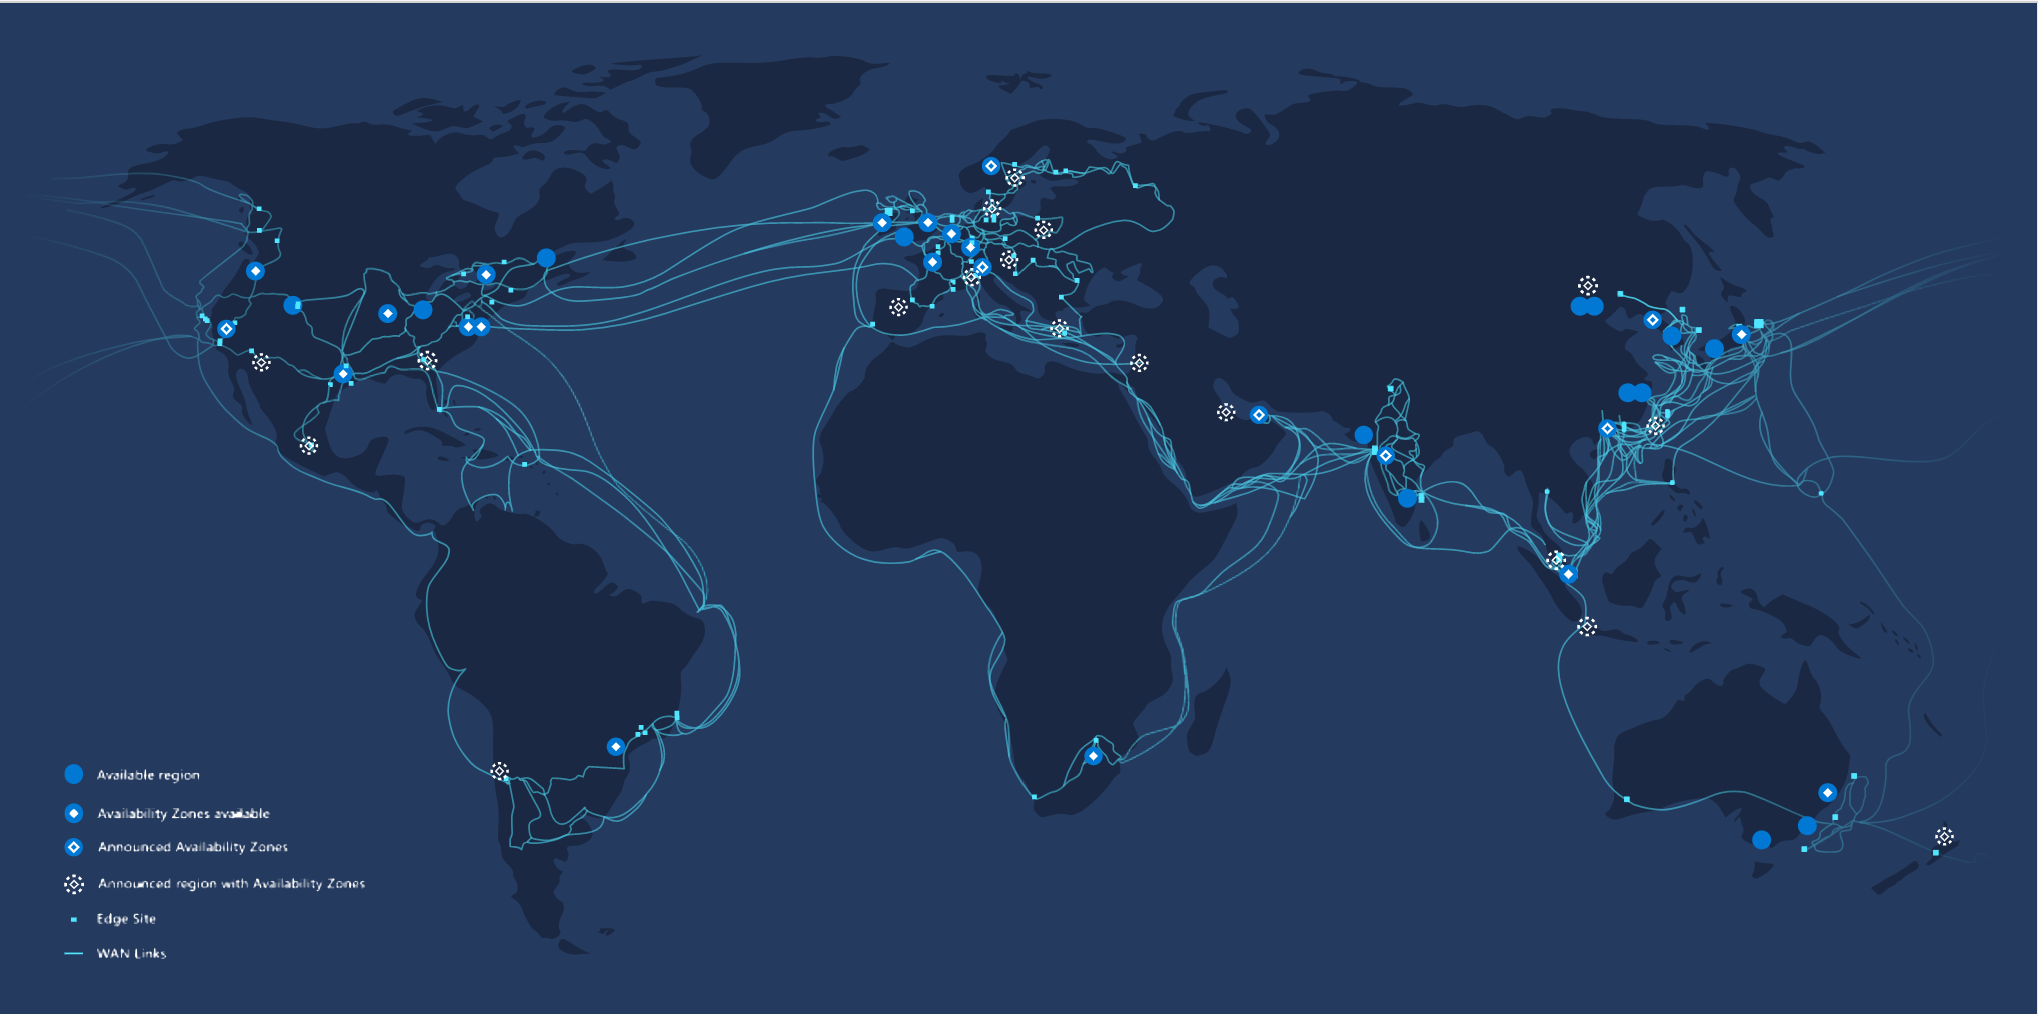
\includegraphics[width=0.9\textwidth]{img/network.png}
    \caption{Data centers and its connection in Azure global network\cite{azure}}
    \label{fig:azure}
\end{figure}

\section{Notation}

In Scheduling Jobs across Geo-Distributed Data Centers, we have a set of jobs and a set of data centers. For each job, there are several tasks. Each task may require data from different centers, and it may also require some data from other tasks of the same job. For each data center, there are some slots to place tasks.

Our assignment is to assign all tasks into slots with the minimum average completion time of these jobs. And we need to make some notations first.

Obviously, we can first denote that there are $K$ jobs and $m$ data centers in total. For job $i$, the number of its tasks is $t_i$. For center $i$, the number of its slots is $s_i$. Then we denote the execution time of task $i$ of job $k$ as $e_{k,i}$. The bandwidth from center $i$ to center $j$ is denoted as $b_{i,j}$. Moreover, $d_{k,i}^j$ denotes the amount of data that task $i$ of job $k$ requires from data center $j$.

Furthermore, for every job $i$, there is a graph $G$ that shows its precedence constraints. And we can use a square matrix $T^i$ to represent it. For example, if task $i_2$ requires data of size $100$ from task $i_1$, then the element $T_{1,2}^i$ will become $100$. If there are no edges between task $i_3$ and $i_4$, then the element $T_{3,4}^i$ will become $0$.

Here is a more specific example. If there are $3$ tasks in job $A$, which we denote as $t_1$, $t_2$ and $t_3$, and $t_2$ needs 100MB data from $t_1$, $t_3$ needs 200MB data from $t_2$, $t_3$ needs 500MB data from $t_1$. Then the corresponding matrix will be:
$$\begin{pmatrix}
0 & 100 & 500 \\
0 & 0 & 200 \\
0 & 0 & 0
\end{pmatrix}$$
Now we have defined the corresponding notations of all the information we know. Finally we will define the variables that we want to optimize.

For every task $i$ of job $k$, we create $m$ binary variables $x_{k,i}^1,\cdots,x_{k,i}^m$. If $x_{k,i}^j=1$, it means task $i$ of job $k$ is allocated to center $j$.

Up to now, we've denoted all the notations we will use in our simulation. Then we need to add constrains to them.

All the variables we denoted are shown in Table \ref{tab:variables}.\\
\begin{table}[h]
    \centering
    \caption{Symbel Table of Variables for Scheduling Jobs Problem}\label{tab:variables}
    \begin{tabular}{c|l}
    \hline
         Variable & Meaning\\
    \hline
        $K$ & The number of jobs\\
        $m$ & The number of data centers\\
        $t_k$ & The number of tasks of job $k$\\
        $s_i$ & The number of slots of center $i$\\
        $e_{k,i}$ & The execution time of task $i$ of job $k$\\
        $b_{i,j}$ & The bandwidth from center $i$ to center $j$\\
        $d_{k,i}^j$ & The amount of data that task $i$ of job $k$ requires from center $j$\\
        $T_{i,j}^k$ & The amount of data that task $j$ of job $k$ requires from task $i$ of job $k$\\
        $q_k$ & The number of stages of job$k$\\
        $p_i^k$ & The number of tasks of stage $i$ of job $k$\\
        $x_{k,i}^j$ & Whether task $i$ of job $k$ is allocated to center $j$\\
        $c_{k,i}$ & The completion time of task $i$ of job $k$\\
        $C_k$ & The completion time of job $k$\\
        $ACT$ & The average completion time of all jobs\\
    \hline
    \end{tabular}
\end{table}

\section{Formalization}
\subsection{Formalization and Test of a Single Example without Max-Min Fairness}

To begin with, we want to simulate a simple example without max min fairness by using Cplex. This example is exactly same as the one introduced in Project-Data-AnalyticJobScheduling.pdf.

\begin{figure}[h]
    \centering
    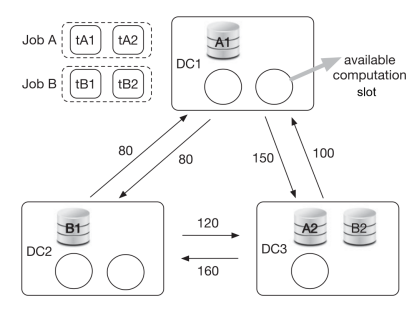
\includegraphics[width=0.4\textwidth]{img/simpleexample.png}
    \caption{An example of scheduling multiple jobs across geo-distributed data centers\cite{Chen2019}}
    \label{fig:azure}
\end{figure}

In this example, we have $K=2$ and $m=3$. There are $2$ parallel tasks for job $A$ and job $B$ each and the execution time for every task is one second. The vector for the number of slots is $\begin{pmatrix}2 & 2 & 1\end{pmatrix}$.\\
The matrix for bandwidth is:
$$\begin{pmatrix}
1000 & 80 & 150 \\
80 & 1000 & 120 \\
100 & 160 & 1000
\end{pmatrix}$$
Moreover, for every job, there is a request matrix.\\
$$D_1=\begin{pmatrix}
100 & 0 & 200 \\
100 & 0 & 200 
\end{pmatrix}
D_2=\begin{pmatrix}
0 & 200 & 200 \\
0 & 200 & 300 
\end{pmatrix}$$
For every job, there is also another matrix with binary elements which is corresponding to $x_{k,i}^j$. Their values need to be determined. Then we need to add constraints.\\
First, for every task $i$ of job $k$, it can only be placed in one single center, which means that 

\begin{equation}\label{eq:one}
    \sum_{j=1}^m x_{k,i}^j=1,\forall i\leq t_i,\forall k\leq K
\end{equation}

Second, for every data center, the number of tasks there could not exceed the number of its slots. Therefore, we have 

\begin{equation}\label{eq:slot}
    \sum_{k=1}^K\sum_{i=1}^{t_k} x_{k,i}^j\leq s_j,\forall j\leq m
\end{equation}

With these constraints, we need to calculate the completion time for each job. Now let's first consider the completion time of a single task. This task may need data from several different centers, and different centers can transfer data to this job concurrently. Therefore, the completion of it will be: 

\begin{equation}\label{eq:task}
    c_{k,i}=\max\limits_{1\leq j_2\leq m}\sum_{j_1=1}^m\frac{x_{k,i}^{j_1}\times d_{k,i}^{j_2}}{b_{j_2,j_1}}+e_{k,i}
\end{equation}

Because every task of a job runs concurrently, we just need to calculate maximal completion time of tasks for every job, which means that $C_k=\max(c_{k,1},\cdots,c_{k,t_k})$. And the average completion time 
\begin{equation}
    ACT=\frac{\sum_{k=1}^K C_k}K
\end{equation}
is what we want to minimize.

Now we have analyzed all the data and constraints of this simple example, then we add data into the file example.dat and add constraints into the file example.mod. We can build a model and simulate this simple example. Here is the result we get:
\begin{figure}[h]
    \centering
    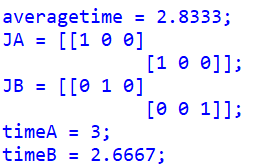
\includegraphics[width=0.3\textwidth]{img/exampleresult.png}
    \caption{Result from simulation of a simple example}
    \label{fig:azure}
\end{figure}

\subsection{Formalization for More Complex Scheduling Jobs Problem}

In the single example, we have made part of formalization of the whole problem. However, there are some constraints that the single example doesn't have.\\
There are only 2 jobs with 2 tasks each in the single example. Moreover, for each job, all of its tasks can run concurrently. But in fact, there may be some precedence constraints inside a job. In part 2 we have defined a matrix to show these precedence constraints. Here we will concentrate on how to use these constraints to calculate corresponding task's completion time.\\
If there exist any precedence constraints inside a job, then we can use a graph $G$ to represent them. For example, if a job has the following graph:
\begin{figure}[h]
    \centering
    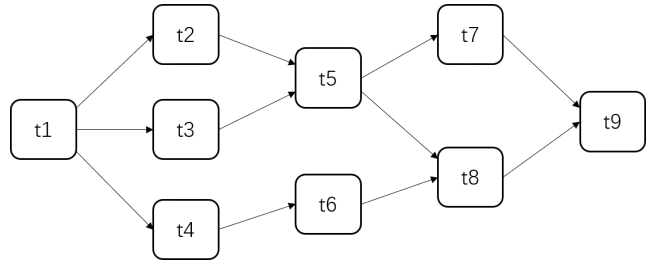
\includegraphics[width=0.5\textwidth]{img/samplegraph.png}
    \caption{An example of a job with precedence constraints}
    \label{fig:azure}
\end{figure}\\
It means that this job has several stages. More importantly, only when an old stage is finished may a new stage start to be computed. In this case, stage $1$ is $\{t1\}$, stage $2$ is $\{t2,t3,t4\}$, stage $3$ is $\{t5,t6\}$, stage $4$ is $\{t7,t8\}$ and stage $5$ is $\{t9\}$.\\
The strategy that we get stages from a graph is: At the beginning, every node is not visited. Then every time we choose the nodes that satisfy the following two requirements to form a new stage. First, these nodes have not been visited. Second, either they don't have parent node or all of their parent nodes have been visited.\\
The completion time of this job, obviously, is the summation of the completion times of its stages. If we define that for job $k$, there are $q_k$ stages in total and the size of each stage $s$ is $p_s^k$, then we have 
\begin{equation}\label{eq:stage}
    C_k=\max(c_{k,1},\cdots,c_{k,p_1^k})+\max(c_{k,p_1^k+1},\cdots,c_{k,p_1^k+p_2^k})+\cdots+\max(c_{k,t_k-p_{q_k}^k+1},\cdots,c_{k,t_k})
\end{equation}

Furthermore, in the simple example, for task $i$ of job $k$, its completion time is the maximal transmission time from a data center to this task plus its execution time. However, after we add precedence constraints, we need to consider the transmission between two tasks and choose the maximal one. So the completion time becomes 
\begin{equation}\label{eq:taske}
    c_{k,i}=\max(\max\limits_{1\leq j_2\leq m}\sum_{j_1=1}^m\frac{x_{k,i}^{j_1}\times d_{k,i}^{j_2}}{b_{j_2,j_1}}+e_{k,i},\max\limits_{1\leq j_3\leq t_k}\sum_{j_1=1}^m\sum_{j_2=1}^m\frac{x_{k,i}^{j_1}\times x_{k,j_3}^{j_2}\times T_{j_3,i}^k}{b_{j_2,j_1}}+e_{k,i})
\end{equation}

where $T_{j_3,i}^k$ is the requested data amount from task $j_3$ to task $i$ in job $k$.

Now there is still a factor that we haven't taken into consideration. In the simple example, there exists a bandwidth between every two data centers. However, in more complex problems, data may be not able to be transferred between some centers directly. In this case, data need to be transferred indirectly. For example, if the bandwidth between center $A$ and center $B$ is 100MB/s and the bandwidth between center $B$ and center $C$ is 100MB/s and there is no bandwidth between center $A$ and center $C$. Then if we want to transform data between $A$ and $C$, we need to transform it indirectly. First, we transform the data from $A$ to $B$, then we transform the data from $B$ to $C$. Moreover, we can calculate the equivalent bandwidth between $A$ and $C$ is 50MB/s.

Using the same strategy, we can calculate the corresponding bandwidth between every two data centers. Considering that the data transferring path need to be optimal, we will use the Floyd-Warshall's Algorithm. The calculating process is: First we calculate every bandwidth's reciprocal, which means the time to transfer 1MB of data through this bandwidth. Then we use Floyd-Warshall Algorithm to the whole matrix. By this way, we can get the optimal time, which is corresponding with optimal path. At last, we turn times into bandwidths by calculating reciprocal again. And we will get a new bandwidth matrix, in which there is also a bandwidth between every two data centers that can transfer data indirectly.

This assumption could be justified by the fact that we could construct a \empty{transfer} task without the need for any computing resources to pass the data from the previous transfer. Because data could transfer on every link, the data could also been transferred indirectly in this way.

\begin{figure}
    \centering
    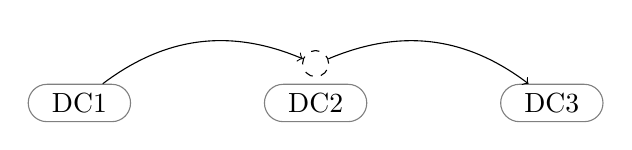
\begin{tikzpicture}[node distance=1cm]
\tikzstyle{dc} = [rounded rectangle,draw=gray,text centered,text width=1cm];
\node[dc] (v1) at (-1,0.5) {DC1};
\node[dc] (v2) at (2,0.5) {DC2};
\node [dc] (v3) at (5,0.5) {DC3};
\node[circle,radius=1cm,draw,dashed] (v4) at (2,1) {};
\draw  (v1) edge[->,bend left] (v4);
\draw  (v4) edge[->,bend left] (v3);
\end{tikzpicture}

    \caption{Indirect transfer through a \emph{transfer} task}
    \label{fig:my_label}
\end{figure}

\subsection{Formalization for Scheduling Jobs with Max-Min Fairness}\label{sec:maxmin}

Finally, we will add description of max min fairness of this problem.

In order to minimize its completion time, every job may require different number of slots from different centers. However, the number of slots for every center is limited. Thus we need max min fairness to determine the allocation.

For each center, if the number of slots that is required from different jobs exceeds the number of slots it has, then we use max-min fairness. 

To satisfy max-min on computing resources, we can first omit the constraints of slots. In this case we will get the number of requests, then we allocate limited slots according to max-min fairness. We will re-allocate the data center that has more requests than demand. For those data centers that has more demand than resources, we will fix the existing allocation in place for the next iteration. In the next iteration, the number of slots in those exceeded data centers will be limited, and apply the minimum average time on the current configuration until all limits on slots are satisfied and we get the optimal solution with minimum average time while maintaining max-min fairness. Figure \ref{fig:maxmin} shows this process intuitively.

Now let's show that by using this strategy, we can reach an approximate max min fairness. For each iteration, we can view the overflowing centers as some small-size glasses with overflowing beer. And we can view the centers with empty slots as some large-size glasses with unfulfilled beer. Then we limit the number of slots in those overflowing centers, run the algorithm again and we will get another allocation. This process is similar to pour that overflowing beer into those glasses with capacity.

How we define a center's capacity of resources is necessary to emphasize here. It doesn't completely depend on the number of its slots. Because for those jobs, one slot may be not so popular as another. Those slots with higher popularity have lower capacity of resources oppositely. And those slots with lower popularity have higher capacity of resources. Therefore, those overflowing centers have more popular slots, correspondingly, they have lower capacity of resources. And we can regard them as glasses with smaller size.

Every time we re-allocate overflowing centers with the constraints of slots, then we lock their allocation, which means that we satisfy glasses of smaller size. We do this iteration again and again until there are no overflowing centers. For each iteration, we still maintain the claim of minimal average completion time, thus the final result with approximate max min fairness will not be too bad. 

% We will firstly satisfy the minimal request, then satisfy the larger requests. If a job's request can not be satisfied, then we will give it a mean value. Because we can only allocate integer values, we can not satisfy max-min fairness strictly. For example, if we want to divide $4$ slots into $3$ groups, then we will get 1,1,2.\\

% According to this scheme, \\

% For example, for center $1$ with $7$ slots, if job $A$ need $2$ slot, job $B$ need $3$ slots and job $C$ need $4$ slots, then the number of slots they get will be 2,2,3.\\

\section{NP-Complete}

This problem is a NP-Complete problem.\cite{10.1145/344588.344618}

The problem is to schedule all the tasks in the DAG to a number of worker nodes --- while minimizing the completion time of the job. Given a set $S$ of all $n$ tasks which can be put into different DAG's, a time limit $k$, a relation $<$ on $S$ which can be determined from the DAG's directed edges and a sequence of integers $c_0,c_1,\ldots,c_{t-1}$ with $\sum_{i=0}^{t-1}{c_i} = n$. Our goal is to find a function $f$ from $S$ to $\{0,1,\ldots,t-1\}$ to make sure that $f^{-1}{(i)}$ has exactly $c_i$ members and make the average cost be minimum.

\begin{definition}[3-Satisfiability --- \textsc{3-SAT}]
Given a set of $\{x_i\}$, $1 \leq i \leq m$, and a collection of sets $D_1,\ldots,D_n$, where $m \leq 3n$, such that each $D_i$ consists of exactly three of the elements $x_i$ or $\overline x_i$.
\end{definition}

Given an instance of \textsc{3-SAT}, we can construct the following instance of this problem. The tasks we shall denote:\\
$x_{ij}$ and $\overline x_{ij}$ for $1 \leq i \leq m$ and $0 \leq j \leq m$;\\
$y_i$ and $\overline y_i$ for $1 \leq i \leq m$;\\
$D_{ij}$ for $1 \leq i \leq n$ and $1 \leq j \leq n$;

Thre relation < is given by:
\begin{enumerate}[(i)]
    \item $x_{ij} < \overline x_{i,j+1}$ and $\overline x_{ij} < \overline x_{i,j+1}$, for $1 \leq i \leq m$ and $0 \leq j < m$;
    \item $x_{i,i-1} < y_i$ and $\overline x_{i,i-1} < \overline y_i$ for $1 \leq i \leq m$;
    \item Considering $D_{ij}$, where $a_1 a_2 a_3$ is the binary representation of $j$.(Note that the case $a_1 = a_2 = a_3$ = 0 can't occur.) Let $D_i$ consist of literals $z_{k_1},z_{k_2},z_{k_3}$, where each $z$ independently stands for $x$ or $\overline x$, in a fixed order. then for $1 \leq p \leq 3$, if $a_p = 1$, we have $\overline z_{k_p,m} < D_{ij}$, where $\overline z$ stands for $\overline x$ or $x$.
\end{enumerate}

The limit of $k$ is $m + 3$, and constants $c_i$, $0 \leq i \leq m + 2$ are:
\begin{align*}
c_0 &= m\\ c_1 &= 2m+1\\ c_i &= 2m+2(i \leq i \leq m)\\ c_{m+1} &= n+m+1\\ c_{m+2} &= 6n    
\end{align*}

We will show that the above instance has a solution if and only if the given instance of \textsc{3-SAT} does. We imagine that $x_i$ or $\overline x_i$ to be true if and only if $x_{i0}$ or $\overline x_{i0}$ is executed at time 0. We know that the presence of the $y$'s and $\overline y$'s forces exactly one of $x_{i0}$ and $\overline x_{i0}$ to be executed at time 1. Then the requirement that $n+m+1$ jobs be executed at time $m+1$ is tantamount to the requirement that for each $i$, there is one $j$ such that $D_{ij}$ may be executed at that time. But this condition is equivalent to saying that the sum of items which $D_i$ represents has value true when those of the $x_i$'s and $\overline x_i$'s which were executed at time 0 are given the value true.

In any solution to the instance, we may not execute both $x_{i0}$ and $\overline x_{i0}$ at time 0 for any $i$. Suppose we did, then since $c_0=m$, there would be some $j$ such that neither $x_{i0}$ nor $\overline x_{i0}$ was executed at time 0. Then neither $y_i$ nor $\overline y_i$ would be executed at or before time $j$, for example, $y_i$ must be preceded by $x_{j0},\ldots,x_{j,j-1}$, each executed strictly before the next in the sequence. The total number of jobs which could be executed at or before time $j$ is thus seen to be:
\begin{enumerate}[(1)]
    \item  at most $m(2j+1)$ of the $x$'s and $\overline x$'s ,that is $z_{0i},\ldots,z_{ij}$ if $z_{i0}$ was executed at time 0 and $z_{i0},\ldots,z_{i,j-1}$
    \item at most $2(j-1)$ of the $y$'s, specially $y_1,\overline y_1,\ldots,\overline y_{j-1}$
\end{enumerate}

We may conclude that in any solution to this instance, exactly one of $x_{i0}$ and $\overline x_{i0}$ is executed at time 0. Moreover, we can determine the exact jobs which are executed at each time, given which of $x_{i0}$ and $\overline x_{i0}$ is executed at time 0. At time t we must execute $z_{it}$ if $z_{i0}$ was executed at time 0 and $z_{i,t-1}$ if not. Moreover, we must execute $y_t$ at time $t$ if $x_{t0}$ was executed at time 0 and execute $y_{t-1}$ at time $t$ if $x_{t0}$ was executed at time 1.

At time m + 1 we can execute the m remaining $x$'s and $\overline x$'s and the one remaining $y$ or $\overline y$. Since $c_{m+1}=m+n+1$, we must be able to execute n of the $D$'s if we are to have a solution. We observe that for each pair $D_{i,j}$ and $D_{i,j'}$, $j \neq j'$, there is at least one $k$ such that $x_{km}$ precedes $D_{ij}$ and $\overline x_{km}$ precedes $D_{ij'}$, or vice versa. Since we have already proven that exactly one of $x_{km}$ and $\overline x_{km}$, can be executed by time m, it follows that for each i, at most one of $D_{i1},\ldots,D_{i7}$ can be executed at time m + 1.

Moreover, if we assign the truth value true to $x_k$ if and only if $x_{k0}$ was executed at time 0, then there will be one of $D_{i1},\ldots,D_{i7}$ executable at time m + 1 if and only if $D_i$ takes the value true under this assignment of values to the variables. We conclude that a solution to the instance  exists if and only if the original product of sums is satisfiable.\cite{ULLMAN1975384}

\begin{equation*}
    \text{\textsc{3-SAT}} \leq_P \text{\textsc{DAG Job Scheduling}}
\end{equation*}
where \textsc{3-SAT} is a NP-Complete problem, so is \textsc{DAG Job Scheduling}.

\section{Algorithm \& Complexity}

The Floyd-Warshall's Algorithm on the bandwidth matrix costs $O(m^3)$, where $m$ is the number of data centers.

For any arbitrary job DAG, to get the stage level of each task, we conduct the following algorithm:
\begin{algorithm}[h]
\caption{DAG Stage Separation}
\KwIn{Request Matrix $D$}
\KwOut{Stage Separation for every job}
Reduce $D$ to $D^\prime$ with task items only\;
Turn $D^\prime$ into adjacency list $G$ on positive element\;
Get topological order of $G$ by recording to \textsc{PRE} of Depth-First Search\;
Run Breadth-First Search on $G$ in topological order to get the stage level, updating the level in a top-down method\;
Group task by (job, level)\;
\end{algorithm}

The algorithm is efficient on parse graph with the use of adjacency list, with the total running time of $O(|V|^2+|E|)$. In this case, $|E|=\Theta(|V|)$, thus $O(|V|^2)$ is the time complexity in this stage, where $|V|=\# tasks=\sum_{k=1}^K\sum_{i=1}^{t_k}1$ is the number of all tasks.

With the stages of each job known, it is time to write down the constraints on elapsed time on each stage. It is discovered that using built-in function \verb"max" in CPLEX is slow. We turned the max function into inequalities. 

Assume that $t_{k,i}$ is denoted as the transmission time from a data center for task $i$ in job $j$ and $t_{k,i}^\prime$ is the transmission time between two tasks for the same task. Equation \eqref{eq:taske} could be turned into

\begin{align}
    c_{k,i} &\geq t_{k,i} + e_{k,i} \label{eq:t1}\\
    c_{k,i} &\geq t_{k,i}^\prime + e_{k,i} \label{eq:t2}\\
    t_{k,i} &\geq \sum_{j_1=1}^m \frac{x_{k,i}^{j_1}\times d_{k,i}^{j_2}}{b_{j_2,j_1}},&& \forall 1\leq j_2\leq m\\
    t_{k,i}^\prime &\geq \sum_{j_1=1}^m\sum_{j_2=1}^m \frac{x_{k,i}^{j_1}\times x_{k,j_3}^{j_2}\times T_{j_3,i}^k}{b_{j_2,j_1}} + e_{k,i},&& \forall 1\leq j_3\leq t_k\label{eq:tend}
\end{align}

It is obvious that to optimze the average cost, $c_{k,i}$ is required to touch the tightest bound in Constraints \eqref{eq:t1} and \eqref{eq:t2}, which satisfies the original equality of \eqref{eq:taske}.

Assume that $c^\prime_{k,s}$ is the cost of stage $s$ in job $k$, then it is the longest cost among all tasks in this stage. And Equation \eqref{eq:stage} is turned into
\begin{align}
    C_k &= \sum_{s=1}^{q_k} c^{\prime}_{k,s} \label{eq:jobm1}\\
    c^\prime_{k,s} &\geq c_{k,i},\quad \forall i: 1+\sum_{l=1}^{s-1} p_{l}^k \leq i \leq \sum_{l=1}^{s} p_{l}^k \label{eq:jobm2}
\end{align}
since the task in every stage could be non-continuous, it is just a representation to show that it is the maximum elapsed time in every stage.

% The time for every iteration process is under 5s in Gurobi, which is efficient enough with thousands of constraints.

To perform the method mentioned in Section \ref{sec:maxmin}, we conduct the iteration algorithm as follows:

\begin{algorithm}[h]
    \caption{Iterative Max-Min Fairness Algorithm}
    Initialize Optimize Model with basic constraints \eqref{eq:one}, (\ref{eq:t1} -- \ref{eq:tend}), (\ref{eq:jobm1} -- \ref{eq:jobm2})\;
    \texttt{ConstrSlot} $\leftarrow$ []\;
    \Repeat{
        original Constraint \eqref{eq:slot} is satisfied
    }{
    \ForEach{\emph{slot}}{
        \eIf{\emph{slot}$\in$\texttt{ConstrSlot}}{
        add constraint on mono \emph{slot} similar to Constraint \eqref{eq:slot}\;
        }
        {
        fix the allocated task on $\emph{slot}$. }
        Optimize Model\;
        append the overflow slots to \texttt{ConstrSlot}\;
        }
    }
\end{algorithm}

The iteration time will not exceed $m$, thus the optimization costs $O(mT)$, where $T$ is the computing cost on Linear Optimization using Gurobi (often 3s).

As a result, the total time complexity of our algorithm is:
\begin{equation*}
    O(m^3)+O(n)+O(mT)
\end{equation*}
where $n=\#tasks$. Our algorithm performs 10s on Toy Data.

\section{Test on Toy Data}
We firstly test the algorithm by using Cplex. However, because we use too many ``max" functions, there is a very large gap between the result and the objective. Then we improve our algorithm and test it by using gurobi. And we get nice results.

The result without max-min fairness is shown in Figure \ref{fig:toydata}, where the left part shows the allocation of tasks and the right part shows the connection between the nodes (red indicates a longer time on transferring). And the result with the iteration process with the max-min allocation on computing resources is shown in Figure \ref{fig:maxmin}, where the upper part is the iteration process and the bottom part shows the change in average time (red line is the time without max-min fairness).

\begin{figure}[h]
    \centering
    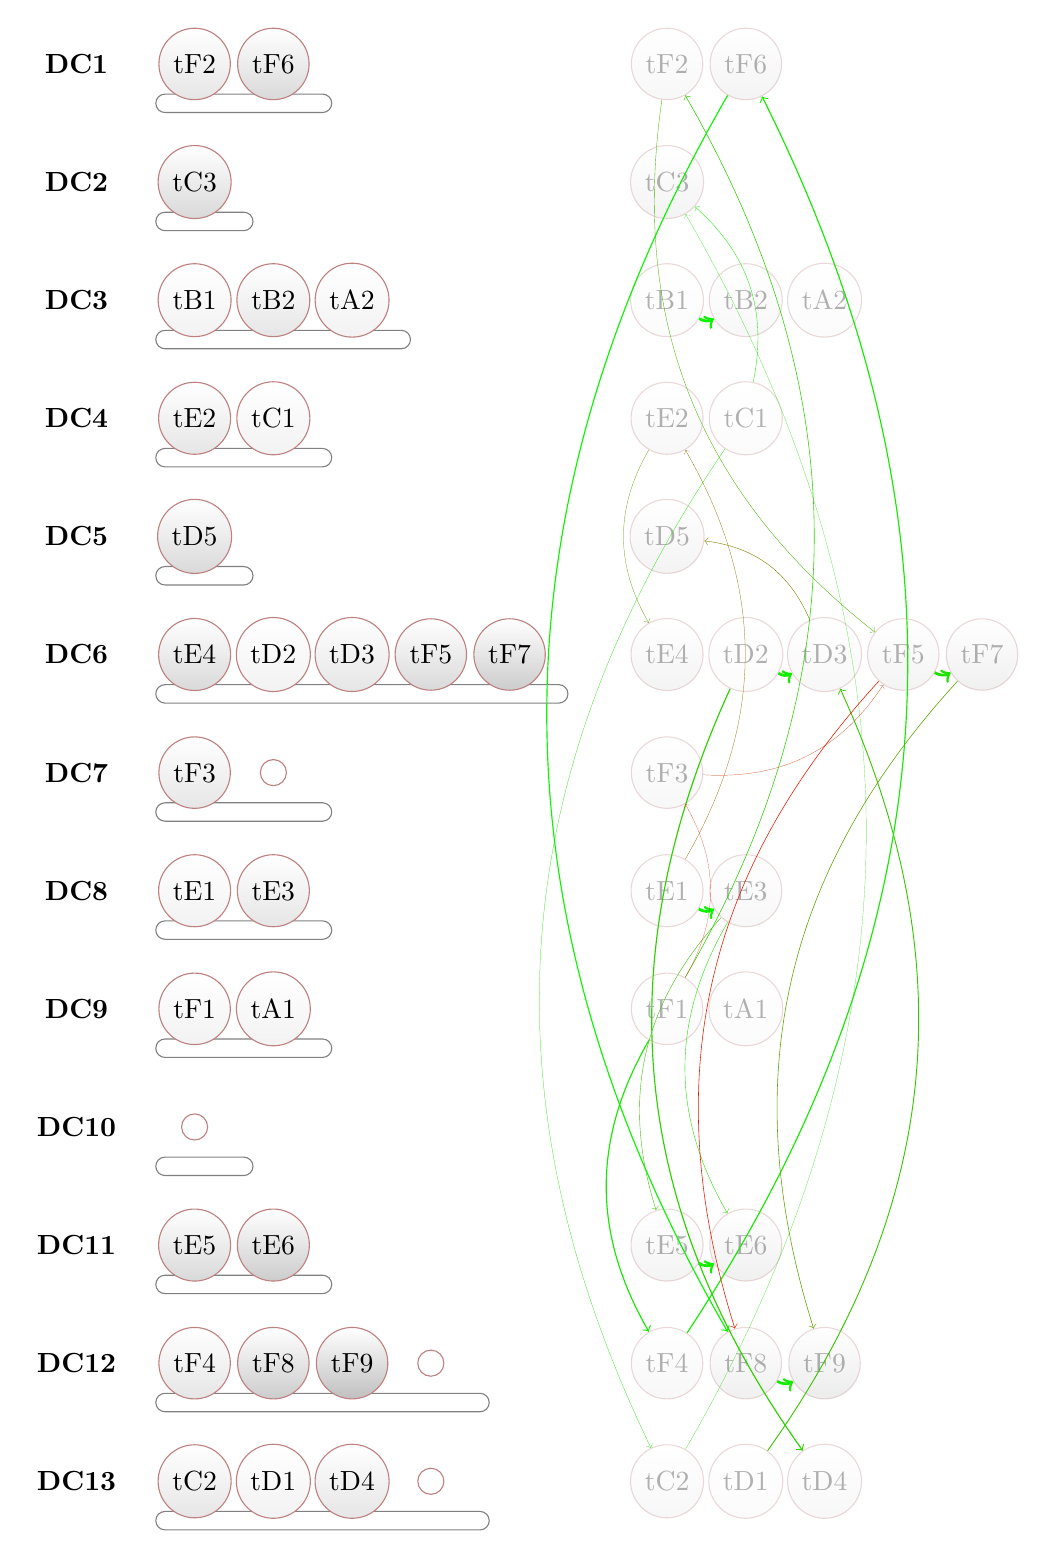
\begin{tikzpicture}

\tikzstyle{dc} = [rounded rectangle,right,draw=gray,yshift=-0.5cm];
\tikzstyle{task} = [circle,draw=red!50!black!50,top color=white];
\node[font=\bfseries] at (-1.5,0) {DC1};
\node[dc,text width=2.0cm] (DC1) at (-0.5,0) {};
\node[task,bottom color=black!10.0] at (0,0) {tF2};
\node[task,bottom color=black!10.0,opacity=0.3] (tF2) at (6,0) {tF2};
\node[task,bottom color=black!15.0] at (1,0) {tF6};
\node[task,bottom color=black!15.0,opacity=0.3] (tF6) at (7,0) {tF6};
\node[font=\bfseries] at (-1.5,-1.5) {DC2};
\node[dc,text width=1.0cm] (DC2) at (-0.5,-1.5) {};
\node[task,bottom color=black!15.0] at (0,-1.5) {tC3};
\node[task,bottom color=black!15.0,opacity=0.3] (tC3) at (6,-1.5) {tC3};
\node[font=\bfseries] at (-1.5,-3.0) {DC3};
\node[dc,text width=3.0cm] (DC3) at (-0.5,-3.0) {};
\node[task,bottom color=black!5.0] at (0,-3.0) {tB1};
\node[task,bottom color=black!5.0,opacity=0.3] (tB1) at (6,-3.0) {tB1};
\node[task,bottom color=black!10.0] at (1,-3.0) {tB2};
\node[task,bottom color=black!10.0,opacity=0.3] (tB2) at (7,-3.0) {tB2};
\node[task,bottom color=black!5.0] at (2,-3.0) {tA2};
\node[task,bottom color=black!5.0,opacity=0.3] (tA2) at (8,-3.0) {tA2};
\node[font=\bfseries] at (-1.5,-4.5) {DC4};
\node[dc,text width=2.0cm] (DC4) at (-0.5,-4.5) {};
\node[task,bottom color=black!10.0] at (0,-4.5) {tE2};
\node[task,bottom color=black!10.0,opacity=0.3] (tE2) at (6,-4.5) {tE2};
\node[task,bottom color=black!5.0] at (1,-4.5) {tC1};
\node[task,bottom color=black!5.0,opacity=0.3] (tC1) at (7,-4.5) {tC1};
\node[font=\bfseries] at (-1.5,-6.0) {DC5};
\node[dc,text width=1.0cm] (DC5) at (-0.5,-6.0) {};
\node[task,bottom color=black!15.0] at (0,-6.0) {tD5};
\node[task,bottom color=black!15.0,opacity=0.3] (tD5) at (6,-6.0) {tD5};
\node[font=\bfseries] at (-1.5,-7.5) {DC6};
\node[dc,text width=5.0cm] (DC6) at (-0.5,-7.5) {};
\node[task,bottom color=black!15.0] at (0,-7.5) {tE4};
\node[task,bottom color=black!15.0,opacity=0.3] (tE4) at (6,-7.5) {tE4};
\node[task,bottom color=black!5.0] at (1,-7.5) {tD2};
\node[task,bottom color=black!5.0,opacity=0.3] (tD2) at (7,-7.5) {tD2};
\node[task,bottom color=black!10.0] at (2,-7.5) {tD3};
\node[task,bottom color=black!10.0,opacity=0.3] (tD3) at (8,-7.5) {tD3};
\node[task,bottom color=black!15.0] at (3,-7.5) {tF5};
\node[task,bottom color=black!15.0,opacity=0.3] (tF5) at (9,-7.5) {tF5};
\node[task,bottom color=black!20.0] at (4,-7.5) {tF7};
\node[task,bottom color=black!20.0,opacity=0.3] (tF7) at (10,-7.5) {tF7};
\node[font=\bfseries] at (-1.5,-9.0) {DC7};
\node[dc,text width=2.0cm] (DC7) at (-0.5,-9.0) {};
\node[task,bottom color=black!10.0] at (0,-9.0) {tF3};
\node[task,bottom color=black!10.0,opacity=0.3] (tF3) at (6,-9.0) {tF3};
\node[task] at (1,-9.0) {};
\node[font=\bfseries] at (-1.5,-10.5) {DC8};
\node[dc,text width=2.0cm] (DC8) at (-0.5,-10.5) {};
\node[task,bottom color=black!5.0] at (0,-10.5) {tE1};
\node[task,bottom color=black!5.0,opacity=0.3] (tE1) at (6,-10.5) {tE1};
\node[task,bottom color=black!10.0] at (1,-10.5) {tE3};
\node[task,bottom color=black!10.0,opacity=0.3] (tE3) at (7,-10.5) {tE3};
\node[font=\bfseries] at (-1.5,-12.0) {DC9};
\node[dc,text width=2.0cm] (DC9) at (-0.5,-12.0) {};
\node[task,bottom color=black!5.0] at (0,-12.0) {tF1};
\node[task,bottom color=black!5.0,opacity=0.3] (tF1) at (6,-12.0) {tF1};
\node[task,bottom color=black!5.0] at (1,-12.0) {tA1};
\node[task,bottom color=black!5.0,opacity=0.3] (tA1) at (7,-12.0) {tA1};
\node[font=\bfseries] at (-1.5,-13.5) {DC10};
\node[dc,text width=1.0cm] (DC10) at (-0.5,-13.5) {};
\node[task] at (0,-13.5) {};
\node[font=\bfseries] at (-1.5,-15.0) {DC11};
\node[dc,text width=2.0cm] (DC11) at (-0.5,-15.0) {};
\node[task,bottom color=black!15.0] at (0,-15.0) {tE5};
\node[task,bottom color=black!15.0,opacity=0.3] (tE5) at (6,-15.0) {tE5};
\node[task,bottom color=black!20.0] at (1,-15.0) {tE6};
\node[task,bottom color=black!20.0,opacity=0.3] (tE6) at (7,-15.0) {tE6};
\node[font=\bfseries] at (-1.5,-16.5) {DC12};
\node[dc,text width=4.0cm] (DC12) at (-0.5,-16.5) {};
\node[task,bottom color=black!10.0] at (0,-16.5) {tF4};
\node[task,bottom color=black!10.0,opacity=0.3] (tF4) at (6,-16.5) {tF4};
\node[task,bottom color=black!20.0] at (1,-16.5) {tF8};
\node[task,bottom color=black!20.0,opacity=0.3] (tF8) at (7,-16.5) {tF8};
\node[task,bottom color=black!25.0] at (2,-16.5) {tF9};
\node[task,bottom color=black!25.0,opacity=0.3] (tF9) at (8,-16.5) {tF9};
\node[task] at (3,-16.5) {};
\node[font=\bfseries] at (-1.5,-18.0) {DC13};
\node[dc,text width=4.0cm] (DC13) at (-0.5,-18.0) {};
\node[task,bottom color=black!10.0] at (0,-18.0) {tC2};
\node[task,bottom color=black!10.0,opacity=0.3] (tC2) at (6,-18.0) {tC2};
\node[task,bottom color=black!5.0] at (1,-18.0) {tD1};
\node[task,bottom color=black!5.0,opacity=0.3] (tD1) at (7,-18.0) {tD1};
\node[task,bottom color=black!10.0] at (2,-18.0) {tD4};
\node[task,bottom color=black!10.0,opacity=0.3] (tD4) at (8,-18.0) {tD4};
\node[task] at (3,-18.0) {};
\draw[red!3.75!green,line width=1.0pt] (tB1) edge[->,bend right] (tB2);
\draw[red!12.15!green,line width=0.09259259259259259pt] (tC1) edge[->,bend right] (tC2);
\draw[red!6.0!green,line width=0.125pt] (tC1) edge[->,bend right] (tC3);
\draw[red!11.75!green,line width=0.06382978723404255pt] (tC2) edge[->,bend right] (tC3);
\draw[red!22.5!green,line width=0.3333333333333333pt] (tD1) edge[->,bend right] (tD3);
\draw[red!7.5!green,line width=1.0pt] (tD2) edge[->,bend right] (tD3);
\draw[red!18.0!green,line width=0.4166666666666667pt] (tD2) edge[->,bend right] (tD4);
\draw[red!50.0!green,line width=0.15pt] (tD3) edge[->,bend right] (tD5);
\draw[red!56.25!green,line width=0.1pt] (tE1) edge[->,bend right] (tE2);
\draw[red!3.0!green,line width=1.0pt] (tE1) edge[->,bend right] (tE3);
\draw[red!37.5!green,line width=0.1pt] (tE2) edge[->,bend right] (tE4);
\draw[red!23.625!green,line width=0.14285714285714285pt] (tE3) edge[->,bend right] (tE5);
\draw[red!13.125!green,line width=0.14285714285714285pt] (tE3) edge[->,bend right] (tE6);
\draw[red!6.75!green,line width=1.0pt] (tE5) edge[->,bend right] (tE6);
\draw[red!18.0!green,line width=0.20833333333333334pt] (tF1) edge[->,bend right] (tF2);
\draw[red!92.10000000000001!green,line width=0.048859934853420196pt] (tF1) edge[->,bend right] (tF3);
\draw[red!9.0!green,line width=0.4166666666666667pt] (tF1) edge[->,bend right] (tF4);
\draw[red!29.25!green,line width=0.1282051282051282pt] (tF2) edge[->,bend right] (tF5);
\draw[red!78.75000000000001!green,line width=0.07142857142857142pt] (tF3) edge[->,bend right] (tF5);
\draw[red!8.1!green,line width=0.4166666666666667pt] (tF4) edge[->,bend right] (tF6);
\draw[red!11.25!green,line width=1.0pt] (tF5) edge[->,bend right] (tF7);
\draw[red!90.0!green,line width=0.20833333333333334pt] (tF5) edge[->,bend right] (tF8);
\draw[red!4.5!green,line width=0.4166666666666667pt] (tF6) edge[->,bend right] (tF8);
\draw[red!36.0!green,line width=0.20833333333333334pt] (tF7) edge[->,bend right] (tF9);
\draw[red!7.5!green,line width=1.0pt] (tF8) edge[->,bend right] (tF9);
\end{tikzpicture}

    \caption{Toy Data Allocation without max-min} % will be replaced by max-min version, program generated graph.
    \label{fig:toydata}
\end{figure}

\begin{figure}[h]
    \centering
    \begin{tabular}{lll}
         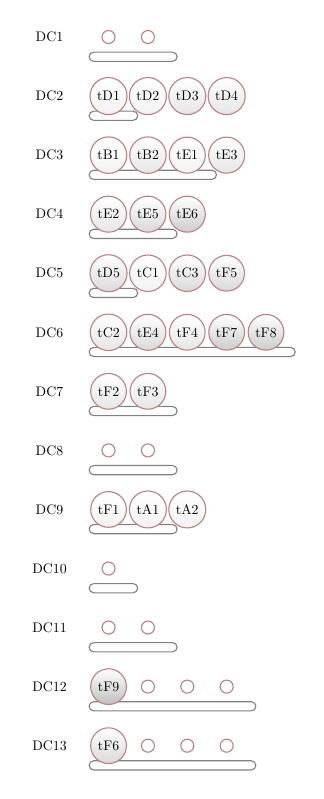
\begin{tikzpicture}[scale=0.5, every node/.style={scale=0.5}]

\tikzstyle{dc} = [rounded rectangle,right,draw=gray,yshift=-0.5cm];
\tikzstyle{task} = [circle,draw=red!50!black!50,top color=white];
\node at (-1.5,0) {DC1};
\node[dc,text width=2.0cm] (DC1) at (-0.5,0) {};
\node[task] at (0,0) {};
\node[task] at (1,0) {};
\node at (-1.5,-1.5) {DC2};
\node[dc,text width=1.0cm] (DC2) at (-0.5,-1.5) {};
\node[task,bottom color=black!5.0] at (0,-1.5) {tD1};
\node[task,bottom color=black!5.0] at (1,-1.5) {tD2};
\node[task,bottom color=black!10.0] at (2,-1.5) {tD3};
\node[task,bottom color=black!10.0] at (3,-1.5) {tD4};
\node at (-1.5,-3.0) {DC3};
\node[dc,text width=3.0cm] (DC3) at (-0.5,-3.0) {};
\node[task,bottom color=black!5.0] at (0,-3.0) {tB1};
\node[task,bottom color=black!10.0] at (1,-3.0) {tB2};
\node[task,bottom color=black!5.0] at (2,-3.0) {tE1};
\node[task,bottom color=black!10.0] at (3,-3.0) {tE3};
\node at (-1.5,-4.5) {DC4};
\node[dc,text width=2.0cm] (DC4) at (-0.5,-4.5) {};
\node[task,bottom color=black!10.0] at (0,-4.5) {tE2};
\node[task,bottom color=black!15.0] at (1,-4.5) {tE5};
\node[task,bottom color=black!20.0] at (2,-4.5) {tE6};
\node at (-1.5,-6.0) {DC5};
\node[dc,text width=1.0cm] (DC5) at (-0.5,-6.0) {};
\node[task,bottom color=black!15.0] at (0,-6.0) {tD5};
\node[task,bottom color=black!5.0] at (1,-6.0) {tC1};
\node[task,bottom color=black!15.0] at (2,-6.0) {tC3};
\node[task,bottom color=black!15.0] at (3,-6.0) {tF5};
\node at (-1.5,-7.5) {DC6};
\node[dc,text width=5.0cm] (DC6) at (-0.5,-7.5) {};
\node[task,bottom color=black!10.0] at (0,-7.5) {tC2};
\node[task,bottom color=black!15.0] at (1,-7.5) {tE4};
\node[task,bottom color=black!10.0] at (2,-7.5) {tF4};
\node[task,bottom color=black!20.0] at (3,-7.5) {tF7};
\node[task,bottom color=black!20.0] at (4,-7.5) {tF8};
\node at (-1.5,-9.0) {DC7};
\node[dc,text width=2.0cm] (DC7) at (-0.5,-9.0) {};
\node[task,bottom color=black!10.0] at (0,-9.0) {tF2};
\node[task,bottom color=black!10.0] at (1,-9.0) {tF3};
\node at (-1.5,-10.5) {DC8};
\node[dc,text width=2.0cm] (DC8) at (-0.5,-10.5) {};
\node[task] at (0,-10.5) {};
\node[task] at (1,-10.5) {};
\node at (-1.5,-12.0) {DC9};
\node[dc,text width=2.0cm] (DC9) at (-0.5,-12.0) {};
\node[task,bottom color=black!5.0] at (0,-12.0) {tF1};
\node[task,bottom color=black!5.0] at (1,-12.0) {tA1};
\node[task,bottom color=black!5.0] at (2,-12.0) {tA2};
\node at (-1.5,-13.5) {DC10};
\node[dc,text width=1.0cm] (DC10) at (-0.5,-13.5) {};
\node[task] at (0,-13.5) {};
\node at (-1.5,-15.0) {DC11};
\node[dc,text width=2.0cm] (DC11) at (-0.5,-15.0) {};
\node[task] at (0,-15.0) {};
\node[task] at (1,-15.0) {};
\node at (-1.5,-16.5) {DC12};
\node[dc,text width=4.0cm] (DC12) at (-0.5,-16.5) {};
\node[task,bottom color=black!25.0] at (0,-16.5) {tF9};
\node[task] at (1,-16.5) {};
\node[task] at (2,-16.5) {};
\node[task] at (3,-16.5) {};
\node at (-1.5,-18.0) {DC13};
\node[dc,text width=4.0cm] (DC13) at (-0.5,-18.0) {};
\node[task,bottom color=black!15.0] at (0,-18.0) {tF6};
\node[task] at (1,-18.0) {};
\node[task] at (2,-18.0) {};
\node[task] at (3,-18.0) {};
\end{tikzpicture}
 & \documentclass[tikz]{standalone}
\usetikzlibrary {positioning,shapes.misc}\begin{document}
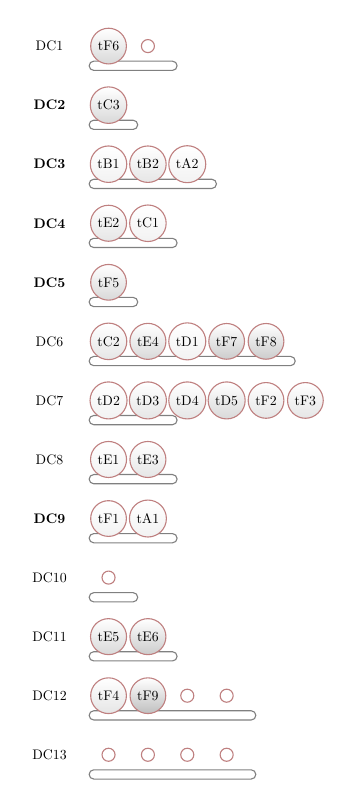
\begin{tikzpicture}[scale=0.5, every node/.style={scale=0.5}]

\tikzstyle{dc} = [rounded rectangle,right,draw=gray,yshift=-0.5cm];
\tikzstyle{task} = [circle,draw=red!50!black!50,top color=white];
\tikzstyle{dp}=[draw,opacity=0.3]
\node at (-1.5,0) {DC1};
\node[dc,text width=2.0cm] (DC1) at (-0.5,0) {};
\node[task,bottom color=black!15.0] at (0,0) {tF6};
\node[task] at (1,0) {};
\node[font=\bfseries] at (-1.5,-1.5) {DC2};
\node[dc,text width=1.0cm] (DC2) at (-0.5,-1.5) {};
\node[task,bottom color=black!15.0] at (0,-1.5) {tC3};
\node[font=\bfseries] at (-1.5,-3.0) {DC3};
\node[dc,text width=3.0cm] (DC3) at (-0.5,-3.0) {};
\node[task,bottom color=black!5.0] at (0,-3.0) {tB1};
\node[task,bottom color=black!10.0] at (1,-3.0) {tB2};
\node[task,bottom color=black!5.0] at (2,-3.0) {tA2};
\node[font=\bfseries] at (-1.5,-4.5) {DC4};
\node[dc,text width=2.0cm] (DC4) at (-0.5,-4.5) {};
\node[task,bottom color=black!10.0] at (0,-4.5) {tE2};
\node[task,bottom color=black!5.0] at (1,-4.5) {tC1};
\node[font=\bfseries] at (-1.5,-6.0) {DC5};
\node[dc,text width=1.0cm] (DC5) at (-0.5,-6.0) {};
\node[task,bottom color=black!15.0] at (0,-6.0) {tF5};
\node at (-1.5,-7.5) {DC6};
\node[dc,text width=5.0cm] (DC6) at (-0.5,-7.5) {};
\node[task,bottom color=black!10.0] at (0,-7.5) {tC2};
\node[task,bottom color=black!15.0] at (1,-7.5) {tE4};
\node[task,bottom color=black!5.0] at (2,-7.5) {tD1};
\node[task,bottom color=black!20.0] at (3,-7.5) {tF7};
\node[task,bottom color=black!20.0] at (4,-7.5) {tF8};
\node at (-1.5,-9.0) {DC7};
\node[dc,text width=2.0cm] (DC7) at (-0.5,-9.0) {};
\node[task,bottom color=black!5.0] at (0,-9.0) {tD2};
\node[task,bottom color=black!10.0] at (1,-9.0) {tD3};
\node[task,bottom color=black!10.0] at (2,-9.0) {tD4};
\node[task,bottom color=black!15.0] at (3,-9.0) {tD5};
\node[task,bottom color=black!10.0] at (4,-9.0) {tF2};
\node[task,bottom color=black!10.0] at (5,-9.0) {tF3};
\node at (-1.5,-10.5) {DC8};
\node[dc,text width=2.0cm] (DC8) at (-0.5,-10.5) {};
\node[task,bottom color=black!5.0] at (0,-10.5) {tE1};
\node[task,bottom color=black!10.0] at (1,-10.5) {tE3};
\node[font=\bfseries] at (-1.5,-12.0) {DC9};
\node[dc,text width=2.0cm] (DC9) at (-0.5,-12.0) {};
\node[task,bottom color=black!5.0] at (0,-12.0) {tF1};
\node[task,bottom color=black!5.0] at (1,-12.0) {tA1};
\node at (-1.5,-13.5) {DC10};
\node[dc,text width=1.0cm] (DC10) at (-0.5,-13.5) {};
\node[task] at (0,-13.5) {};
\node at (-1.5,-15.0) {DC11};
\node[dc,text width=2.0cm] (DC11) at (-0.5,-15.0) {};
\node[task,bottom color=black!15.0] at (0,-15.0) {tE5};
\node[task,bottom color=black!20.0] at (1,-15.0) {tE6};
\node at (-1.5,-16.5) {DC12};
\node[dc,text width=4.0cm] (DC12) at (-0.5,-16.5) {};
\node[task,bottom color=black!10.0] at (0,-16.5) {tF4};
\node[task,bottom color=black!25.0] at (1,-16.5) {tF9};
\node[task] at (2,-16.5) {};
\node[task] at (3,-16.5) {};
\node at (-1.5,-18.0) {DC13};
\node[dc,text width=4.0cm] (DC13) at (-0.5,-18.0) {};
\node[task] at (0,-18.0) {};
\node[task] at (1,-18.0) {};
\node[task] at (2,-18.0) {};
\node[task] at (3,-18.0) {};
\end{tikzpicture}
\end{document}
 &  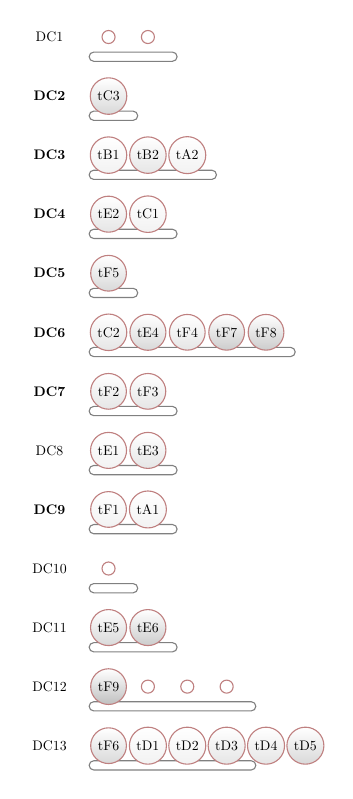
\begin{tikzpicture}[scale=0.5, every node/.style={scale=0.5}]

\tikzstyle{dc} = [rounded rectangle,right,draw=gray,yshift=-0.5cm];
\tikzstyle{task} = [circle,draw=red!50!black!50,top color=white];
\tikzstyle{dp}=[draw,opacity=0.3]
\node at (-1.5,0) {DC1};
\node[dc,text width=2.0cm] (DC1) at (-0.5,0) {};
\node[task] at (0,0) {};
\node[task] at (1,0) {};
\node[font=\bfseries] at (-1.5,-1.5) {DC2};
\node[dc,text width=1.0cm] (DC2) at (-0.5,-1.5) {};
\node[task,bottom color=black!15.0] at (0,-1.5) {tC3};
\node[font=\bfseries] at (-1.5,-3.0) {DC3};
\node[dc,text width=3.0cm] (DC3) at (-0.5,-3.0) {};
\node[task,bottom color=black!5.0] at (0,-3.0) {tB1};
\node[task,bottom color=black!10.0] at (1,-3.0) {tB2};
\node[task,bottom color=black!5.0] at (2,-3.0) {tA2};
\node[font=\bfseries] at (-1.5,-4.5) {DC4};
\node[dc,text width=2.0cm] (DC4) at (-0.5,-4.5) {};
\node[task,bottom color=black!10.0] at (0,-4.5) {tE2};
\node[task,bottom color=black!5.0] at (1,-4.5) {tC1};
\node[font=\bfseries] at (-1.5,-6.0) {DC5};
\node[dc,text width=1.0cm] (DC5) at (-0.5,-6.0) {};
\node[task,bottom color=black!15.0] at (0,-6.0) {tF5};
\node[font=\bfseries] at (-1.5,-7.5) {DC6};
\node[dc,text width=5.0cm] (DC6) at (-0.5,-7.5) {};
\node[task,bottom color=black!10.0] at (0,-7.5) {tC2};
\node[task,bottom color=black!15.0] at (1,-7.5) {tE4};
\node[task,bottom color=black!10.0] at (2,-7.5) {tF4};
\node[task,bottom color=black!20.0] at (3,-7.5) {tF7};
\node[task,bottom color=black!20.0] at (4,-7.5) {tF8};
\node[font=\bfseries] at (-1.5,-9.0) {DC7};
\node[dc,text width=2.0cm] (DC7) at (-0.5,-9.0) {};
\node[task,bottom color=black!10.0] at (0,-9.0) {tF2};
\node[task,bottom color=black!10.0] at (1,-9.0) {tF3};
\node at (-1.5,-10.5) {DC8};
\node[dc,text width=2.0cm] (DC8) at (-0.5,-10.5) {};
\node[task,bottom color=black!5.0] at (0,-10.5) {tE1};
\node[task,bottom color=black!10.0] at (1,-10.5) {tE3};
\node[font=\bfseries] at (-1.5,-12.0) {DC9};
\node[dc,text width=2.0cm] (DC9) at (-0.5,-12.0) {};
\node[task,bottom color=black!5.0] at (0,-12.0) {tF1};
\node[task,bottom color=black!5.0] at (1,-12.0) {tA1};
\node at (-1.5,-13.5) {DC10};
\node[dc,text width=1.0cm] (DC10) at (-0.5,-13.5) {};
\node[task] at (0,-13.5) {};
\node at (-1.5,-15.0) {DC11};
\node[dc,text width=2.0cm] (DC11) at (-0.5,-15.0) {};
\node[task,bottom color=black!15.0] at (0,-15.0) {tE5};
\node[task,bottom color=black!20.0] at (1,-15.0) {tE6};
\node at (-1.5,-16.5) {DC12};
\node[dc,text width=4.0cm] (DC12) at (-0.5,-16.5) {};
\node[task,bottom color=black!25.0] at (0,-16.5) {tF9};
\node[task] at (1,-16.5) {};
\node[task] at (2,-16.5) {};
\node[task] at (3,-16.5) {};
\node at (-1.5,-18.0) {DC13};
\node[dc,text width=4.0cm] (DC13) at (-0.5,-18.0) {};
\node[task,bottom color=black!15.0] at (0,-18.0) {tF6};
\node[task,bottom color=black!5.0] at (1,-18.0) {tD1};
\node[task,bottom color=black!5.0] at (2,-18.0) {tD2};
\node[task,bottom color=black!10.0] at (3,-18.0) {tD3};
\node[task,bottom color=black!10.0] at (4,-18.0) {tD4};
\node[task,bottom color=black!15.0] at (5,-18.0) {tD5};
\end{tikzpicture}
\\
         \hspace*{2em} Iteration 0 & \hspace*{2em} Iteration 1  &\hspace*{2em} Iteration 2 \\
     & 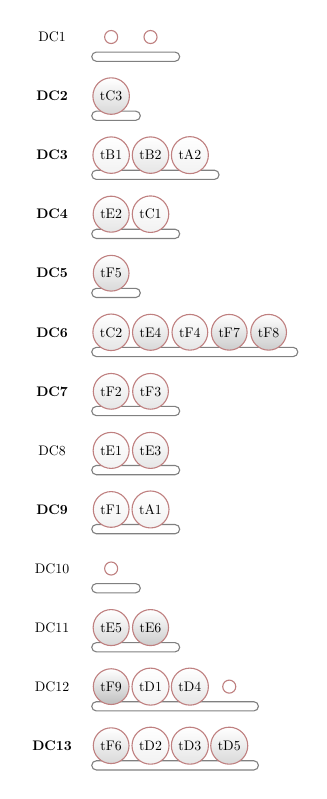
\begin{tikzpicture}[scale=0.5, every node/.style={scale=0.5}]

\tikzstyle{dc} = [rounded rectangle,right,draw=gray,yshift=-0.5cm];
\tikzstyle{task} = [circle,draw=red!50!black!50,top color=white];
\tikzstyle{dp}=[draw,opacity=0.3]
\node at (-1.5,0) {DC1};
\node[dc,text width=2.0cm] (DC1) at (-0.5,0) {};
\node[task] at (0,0) {};
\node[task] at (1,0) {};
\node[font=\bfseries] at (-1.5,-1.5) {DC2};
\node[dc,text width=1.0cm] (DC2) at (-0.5,-1.5) {};
\node[task,bottom color=black!15.0] at (0,-1.5) {tC3};
\node[font=\bfseries] at (-1.5,-3.0) {DC3};
\node[dc,text width=3.0cm] (DC3) at (-0.5,-3.0) {};
\node[task,bottom color=black!5.0] at (0,-3.0) {tB1};
\node[task,bottom color=black!10.0] at (1,-3.0) {tB2};
\node[task,bottom color=black!5.0] at (2,-3.0) {tA2};
\node[font=\bfseries] at (-1.5,-4.5) {DC4};
\node[dc,text width=2.0cm] (DC4) at (-0.5,-4.5) {};
\node[task,bottom color=black!10.0] at (0,-4.5) {tE2};
\node[task,bottom color=black!5.0] at (1,-4.5) {tC1};
\node[font=\bfseries] at (-1.5,-6.0) {DC5};
\node[dc,text width=1.0cm] (DC5) at (-0.5,-6.0) {};
\node[task,bottom color=black!15.0] at (0,-6.0) {tF5};
\node[font=\bfseries] at (-1.5,-7.5) {DC6};
\node[dc,text width=5.0cm] (DC6) at (-0.5,-7.5) {};
\node[task,bottom color=black!10.0] at (0,-7.5) {tC2};
\node[task,bottom color=black!15.0] at (1,-7.5) {tE4};
\node[task,bottom color=black!10.0] at (2,-7.5) {tF4};
\node[task,bottom color=black!20.0] at (3,-7.5) {tF7};
\node[task,bottom color=black!20.0] at (4,-7.5) {tF8};
\node[font=\bfseries] at (-1.5,-9.0) {DC7};
\node[dc,text width=2.0cm] (DC7) at (-0.5,-9.0) {};
\node[task,bottom color=black!10.0] at (0,-9.0) {tF2};
\node[task,bottom color=black!10.0] at (1,-9.0) {tF3};
\node at (-1.5,-10.5) {DC8};
\node[dc,text width=2.0cm] (DC8) at (-0.5,-10.5) {};
\node[task,bottom color=black!5.0] at (0,-10.5) {tE1};
\node[task,bottom color=black!10.0] at (1,-10.5) {tE3};
\node[font=\bfseries] at (-1.5,-12.0) {DC9};
\node[dc,text width=2.0cm] (DC9) at (-0.5,-12.0) {};
\node[task,bottom color=black!5.0] at (0,-12.0) {tF1};
\node[task,bottom color=black!5.0] at (1,-12.0) {tA1};
\node at (-1.5,-13.5) {DC10};
\node[dc,text width=1.0cm] (DC10) at (-0.5,-13.5) {};
\node[task] at (0,-13.5) {};
\node at (-1.5,-15.0) {DC11};
\node[dc,text width=2.0cm] (DC11) at (-0.5,-15.0) {};
\node[task,bottom color=black!15.0] at (0,-15.0) {tE5};
\node[task,bottom color=black!20.0] at (1,-15.0) {tE6};
\node at (-1.5,-16.5) {DC12};
\node[dc,text width=4.0cm] (DC12) at (-0.5,-16.5) {};
\node[task,bottom color=black!25.0] at (0,-16.5) {tF9};
\node[task,bottom color=black!5.0] at (1,-16.5) {tD1};
\node[task,bottom color=black!10.0] at (2,-16.5) {tD4};
\node[task] at (3,-16.5) {};
\node[font=\bfseries] at (-1.5,-18.0) {DC13};
\node[dc,text width=4.0cm] (DC13) at (-0.5,-18.0) {};
\node[task,bottom color=black!15.0] at (0,-18.0) {tF6};
\node[task,bottom color=black!5.0] at (1,-18.0) {tD2};
\node[task,bottom color=black!10.0] at (2,-18.0) {tD3};
\node[task,bottom color=black!15.0] at (3,-18.0) {tD5};
\end{tikzpicture}
 & \documentclass[tikz]{standalone}
\begin{document}
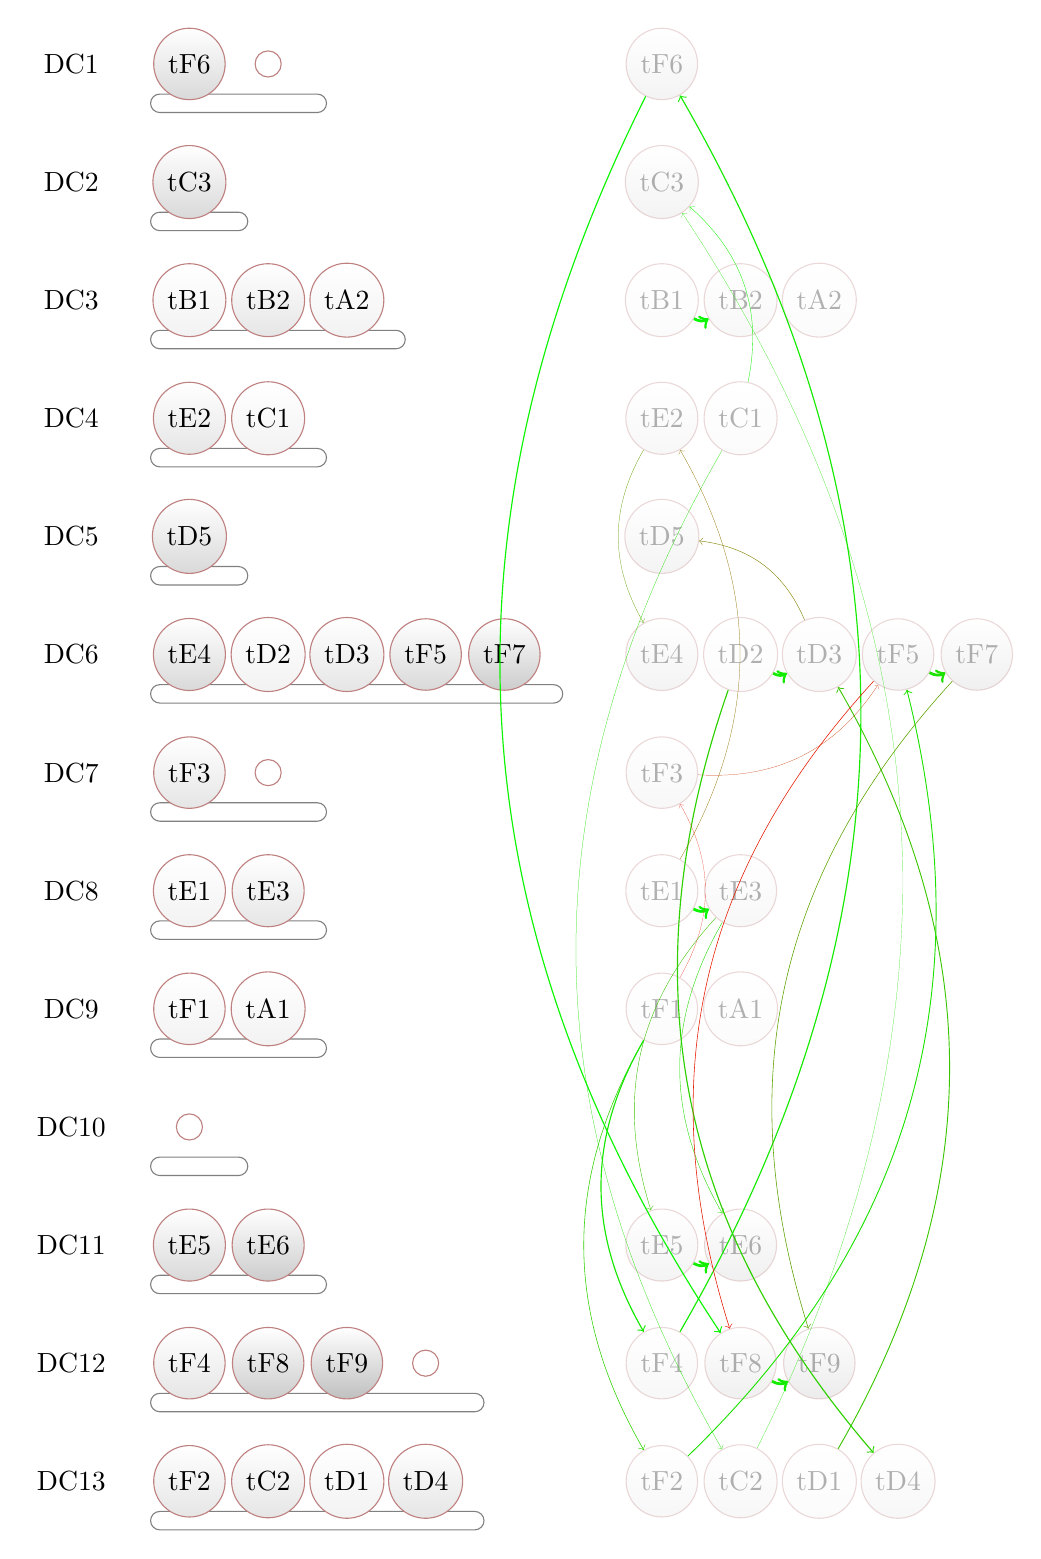
\begin{tikzpicture}
\usetikzlibrary {positioning,shapes.misc}
\tikzstyle{dc} = [rounded rectangle,right,draw=gray,yshift=-0.5cm];
\tikzstyle{task} = [circle,draw=red!50!black!50,top color=white];
\node at (-1.5,0) {DC1};
\node[dc,text width=2.0cm] (DC1) at (-0.5,0) {};
\node[task,bottom color=black!15.0] at (0,0) {tF6};
\node[task,bottom color=black!15.0,opacity=0.3] (tF6) at (6,0) {tF6};
\node[task] at (1,0) {};
\node at (-1.5,-1.5) {DC2};
\node[dc,text width=1.0cm] (DC2) at (-0.5,-1.5) {};
\node[task,bottom color=black!15.0] at (0,-1.5) {tC3};
\node[task,bottom color=black!15.0,opacity=0.3] (tC3) at (6,-1.5) {tC3};
\node at (-1.5,-3.0) {DC3};
\node[dc,text width=3.0cm] (DC3) at (-0.5,-3.0) {};
\node[task,bottom color=black!5.0] at (0,-3.0) {tB1};
\node[task,bottom color=black!5.0,opacity=0.3] (tB1) at (6,-3.0) {tB1};
\node[task,bottom color=black!10.0] at (1,-3.0) {tB2};
\node[task,bottom color=black!10.0,opacity=0.3] (tB2) at (7,-3.0) {tB2};
\node[task,bottom color=black!5.0] at (2,-3.0) {tA2};
\node[task,bottom color=black!5.0,opacity=0.3] (tA2) at (8,-3.0) {tA2};
\node at (-1.5,-4.5) {DC4};
\node[dc,text width=2.0cm] (DC4) at (-0.5,-4.5) {};
\node[task,bottom color=black!10.0] at (0,-4.5) {tE2};
\node[task,bottom color=black!10.0,opacity=0.3] (tE2) at (6,-4.5) {tE2};
\node[task,bottom color=black!5.0] at (1,-4.5) {tC1};
\node[task,bottom color=black!5.0,opacity=0.3] (tC1) at (7,-4.5) {tC1};
\node at (-1.5,-6.0) {DC5};
\node[dc,text width=1.0cm] (DC5) at (-0.5,-6.0) {};
\node[task,bottom color=black!15.0] at (0,-6.0) {tD5};
\node[task,bottom color=black!15.0,opacity=0.3] (tD5) at (6,-6.0) {tD5};
\node at (-1.5,-7.5) {DC6};
\node[dc,text width=5.0cm] (DC6) at (-0.5,-7.5) {};
\node[task,bottom color=black!15.0] at (0,-7.5) {tE4};
\node[task,bottom color=black!15.0,opacity=0.3] (tE4) at (6,-7.5) {tE4};
\node[task,bottom color=black!5.0] at (1,-7.5) {tD2};
\node[task,bottom color=black!5.0,opacity=0.3] (tD2) at (7,-7.5) {tD2};
\node[task,bottom color=black!10.0] at (2,-7.5) {tD3};
\node[task,bottom color=black!10.0,opacity=0.3] (tD3) at (8,-7.5) {tD3};
\node[task,bottom color=black!15.0] at (3,-7.5) {tF5};
\node[task,bottom color=black!15.0,opacity=0.3] (tF5) at (9,-7.5) {tF5};
\node[task,bottom color=black!20.0] at (4,-7.5) {tF7};
\node[task,bottom color=black!20.0,opacity=0.3] (tF7) at (10,-7.5) {tF7};
\node at (-1.5,-9.0) {DC7};
\node[dc,text width=2.0cm] (DC7) at (-0.5,-9.0) {};
\node[task,bottom color=black!10.0] at (0,-9.0) {tF3};
\node[task,bottom color=black!10.0,opacity=0.3] (tF3) at (6,-9.0) {tF3};
\node[task] at (1,-9.0) {};
\node at (-1.5,-10.5) {DC8};
\node[dc,text width=2.0cm] (DC8) at (-0.5,-10.5) {};
\node[task,bottom color=black!5.0] at (0,-10.5) {tE1};
\node[task,bottom color=black!5.0,opacity=0.3] (tE1) at (6,-10.5) {tE1};
\node[task,bottom color=black!10.0] at (1,-10.5) {tE3};
\node[task,bottom color=black!10.0,opacity=0.3] (tE3) at (7,-10.5) {tE3};
\node at (-1.5,-12.0) {DC9};
\node[dc,text width=2.0cm] (DC9) at (-0.5,-12.0) {};
\node[task,bottom color=black!5.0] at (0,-12.0) {tF1};
\node[task,bottom color=black!5.0,opacity=0.3] (tF1) at (6,-12.0) {tF1};
\node[task,bottom color=black!5.0] at (1,-12.0) {tA1};
\node[task,bottom color=black!5.0,opacity=0.3] (tA1) at (7,-12.0) {tA1};
\node at (-1.5,-13.5) {DC10};
\node[dc,text width=1.0cm] (DC10) at (-0.5,-13.5) {};
\node[task] at (0,-13.5) {};
\node at (-1.5,-15.0) {DC11};
\node[dc,text width=2.0cm] (DC11) at (-0.5,-15.0) {};
\node[task,bottom color=black!15.0] at (0,-15.0) {tE5};
\node[task,bottom color=black!15.0,opacity=0.3] (tE5) at (6,-15.0) {tE5};
\node[task,bottom color=black!20.0] at (1,-15.0) {tE6};
\node[task,bottom color=black!20.0,opacity=0.3] (tE6) at (7,-15.0) {tE6};
\node at (-1.5,-16.5) {DC12};
\node[dc,text width=4.0cm] (DC12) at (-0.5,-16.5) {};
\node[task,bottom color=black!10.0] at (0,-16.5) {tF4};
\node[task,bottom color=black!10.0,opacity=0.3] (tF4) at (6,-16.5) {tF4};
\node[task,bottom color=black!20.0] at (1,-16.5) {tF8};
\node[task,bottom color=black!20.0,opacity=0.3] (tF8) at (7,-16.5) {tF8};
\node[task,bottom color=black!25.0] at (2,-16.5) {tF9};
\node[task,bottom color=black!25.0,opacity=0.3] (tF9) at (8,-16.5) {tF9};
\node[task] at (3,-16.5) {};
\node at (-1.5,-18.0) {DC13};
\node[dc,text width=4.0cm] (DC13) at (-0.5,-18.0) {};
\node[task,bottom color=black!10.0] at (0,-18.0) {tF2};
\node[task,bottom color=black!10.0,opacity=0.3] (tF2) at (6,-18.0) {tF2};
\node[task,bottom color=black!10.0] at (1,-18.0) {tC2};
\node[task,bottom color=black!10.0,opacity=0.3] (tC2) at (7,-18.0) {tC2};
\node[task,bottom color=black!5.0] at (2,-18.0) {tD1};
\node[task,bottom color=black!5.0,opacity=0.3] (tD1) at (8,-18.0) {tD1};
\node[task,bottom color=black!10.0] at (3,-18.0) {tD4};
\node[task,bottom color=black!10.0,opacity=0.3] (tD4) at (9,-18.0) {tD4};
\draw[red!3.75!green,line width=1.0pt] (tB1) edge[->,bend right] (tB2);
\draw[red!12.15!green,line width=0.09259259259259259pt] (tC1) edge[->,bend right] (tC2);
\draw[red!6.0!green,line width=0.125pt] (tC1) edge[->,bend right] (tC3);
\draw[red!11.75!green,line width=0.06382978723404255pt] (tC2) edge[->,bend right] (tC3);
\draw[red!22.5!green,line width=0.3333333333333333pt] (tD1) edge[->,bend right] (tD3);
\draw[red!7.5!green,line width=1.0pt] (tD2) edge[->,bend right] (tD3);
\draw[red!18.0!green,line width=0.4166666666666667pt] (tD2) edge[->,bend right] (tD4);
\draw[red!50.0!green,line width=0.15pt] (tD3) edge[->,bend right] (tD5);
\draw[red!56.25!green,line width=0.1pt] (tE1) edge[->,bend right] (tE2);
\draw[red!3.0!green,line width=1.0pt] (tE1) edge[->,bend right] (tE3);
\draw[red!37.5!green,line width=0.1pt] (tE2) edge[->,bend right] (tE4);
\draw[red!23.625!green,line width=0.14285714285714285pt] (tE3) edge[->,bend right] (tE5);
\draw[red!13.125!green,line width=0.14285714285714285pt] (tE3) edge[->,bend right] (tE6);
\draw[red!6.75!green,line width=1.0pt] (tE5) edge[->,bend right] (tE6);
\draw[red!18.0!green,line width=0.20833333333333334pt] (tF1) edge[->,bend right] (tF2);
\draw[red!92.10000000000001!green,line width=0.048859934853420196pt] (tF1) edge[->,bend right] (tF3);
\draw[red!9.0!green,line width=0.4166666666666667pt] (tF1) edge[->,bend right] (tF4);
\draw[red!11.25!green,line width=0.3333333333333333pt] (tF2) edge[->,bend right] (tF5);
\draw[red!78.75000000000001!green,line width=0.07142857142857142pt] (tF3) edge[->,bend right] (tF5);
\draw[red!8.1!green,line width=0.4166666666666667pt] (tF4) edge[->,bend right] (tF6);
\draw[red!11.25!green,line width=1.0pt] (tF5) edge[->,bend right] (tF7);
\draw[red!90.0!green,line width=0.20833333333333334pt] (tF5) edge[->,bend right] (tF8);
\draw[red!4.5!green,line width=0.4166666666666667pt] (tF6) edge[->,bend right] (tF8);
\draw[red!36.0!green,line width=0.20833333333333334pt] (tF7) edge[->,bend right] (tF9);
\draw[red!7.5!green,line width=1.0pt] (tF8) edge[->,bend right] (tF9);
\end{tikzpicture}
\end{document}
\\
         & \hspace*{2em} Iteration 3 &\hspace*{2em} Iteration 4 \\
    \end{tabular}
    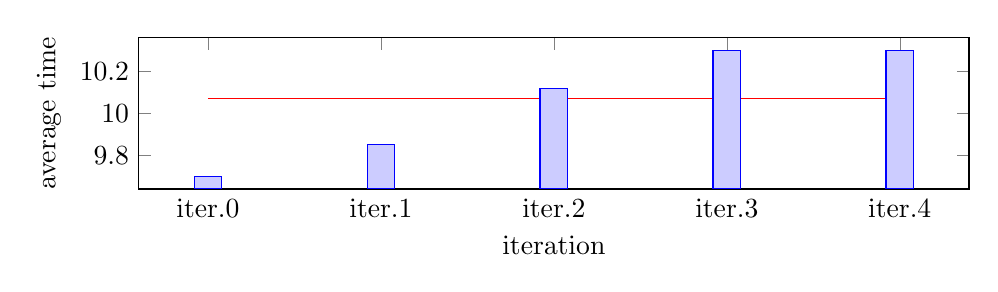
\begin{tikzpicture}
\begin{axis}[xlabel={iteration},
ylabel={average time},
symbolic x coords={iter.0,iter.1,iter.2,iter.3,iter.4},
width=\textwidth,
height=3.5cm,
xtick=data % important
]
%  \addplot+ [ybar,no markers,fill=blue!20,] coordinates { (naive,10.073)};
  \draw[red]
        (axis cs:iter.0,10.073)
        --  (axis cs:iter.4, 10.073)
    ;
 \addplot+ [ybar,no markers,fill=blue!20,] coordinates { (iter.0,9.701) (iter.1,9.854) (iter.2,10.118) (iter.3,10.301) (iter.4,10.301)};
\end{axis}
\end{tikzpicture}

    \caption{Max-min iteration}
    \label{fig:maxmin}
\end{figure}

% \begin{table}
%     \centering
%     \begin{tabular}{c|rrrrr}
%                     &  without Max-min & Iter. 0 & Iter. 1 & Iter.2  & Iter. 3\\
%         Average Time & 2.239 & 2.156 & 2.190 & 2.289 & 2.289 \\
%     \end{tabular}
%     \caption{Average Time}
%     \label{tab:my_label}
% \end{table}


\section{Test on Real World Data}

% The real world bandwidth is based on \cite{Chen2019}, shown in Table \ref{tab:bandwidth}. 

% \begin{table}[h]
%     \centering
%     \caption{Available bandwidth across Geo-Based Data Centers}\label{tab:bandwidth}
%     \begin{tabular}{c|cccccc}
%     \hline
%          & Virginia & Oregon & Ireland & Singapore & Sydney & San Paulo\\
%     \hline
%         Virginia & 1000 & 169 & 154&  52& 53& 104 \\
%         Oregon & - & 1000 & 71 & 69 &  77 & 68 \\
%         Ireland & - & - & 1000& 49 & 40 & 65 \\
%         Singapore & -& -& -& 1000& 58& 35 \\
%         Sydney & -& - &-& -& 1000& 38 \\
%         San Paulo & -& -& -& -& -& 1000 \\
%     \hline
%     \end{tabular}
% \end{table}

Real world should satisfy that the total number of slots is larger than or equal to the total number of tasks, which means that $\sum_{i=1}^m s_i\geq \sum_{i=1}^K t_i$. In order to meet the requirement of this problem, we generate a certain amount of data sets according to certain constraints to test and check our algorithm. In our test sets, all of the data are generated by random numbers.

For bandwidth, because it takes almost no time to transfer data in the same data center, its bandwidth is set to be much larger than other bandwidth values. Other bandwidth is set according to $50\%$ generation probability. For the required data amounts between tasks and datasets, the corresponding demand path is generated according to $20\%$ probability. For every job's tasks, the generation probability of each directed acyclic edge is set to be $20\%$. Other data in the data set is set according to its possible and reasonable range to ensure that it conforms to the real situation.

Figure \ref{fig:real} shows the simulation result with the double data scale. The running time is 15s, which indicates that our algorithm is efficient enough.

\begin{figure}[h]
    \centering
    \begin{tabular}{lll}
         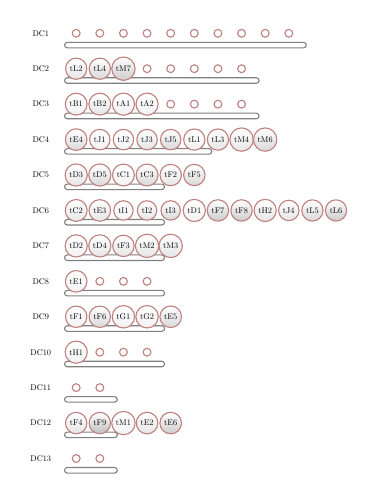
\begin{tikzpicture}[scale=0.3, every node/.style={scale=0.3}]

\tikzstyle{dc} = [rounded rectangle,right,draw=gray,yshift=-0.5cm];
\tikzstyle{task} = [circle,draw=red!50!black!50,top color=white];
\tikzstyle{dp}=[draw,opacity=0.3]
\node at (-1.5,0) {DC1};
\node[dc,text width=10.0cm] (DC1) at (-0.5,0) {};
\node[task] at (0,0) {};
\node[task] at (1,0) {};
\node[task] at (2,0) {};
\node[task] at (3,0) {};
\node[task] at (4,0) {};
\node[task] at (5,0) {};
\node[task] at (6,0) {};
\node[task] at (7,0) {};
\node[task] at (8,0) {};
\node[task] at (9,0) {};
\node at (-1.5,-1.5) {DC2};
\node[dc,text width=8.0cm] (DC2) at (-0.5,-1.5) {};
\node[task,bottom color=black!10.0] at (0,-1.5) {tL2};
\node[task,bottom color=black!15.0] at (1,-1.5) {tL4};
\node[task,bottom color=black!20.0] at (2,-1.5) {tM7};
\node[task] at (3,-1.5) {};
\node[task] at (4,-1.5) {};
\node[task] at (5,-1.5) {};
\node[task] at (6,-1.5) {};
\node[task] at (7,-1.5) {};
\node at (-1.5,-3.0) {DC3};
\node[dc,text width=8.0cm] (DC3) at (-0.5,-3.0) {};
\node[task,bottom color=black!5.0] at (0,-3.0) {tB1};
\node[task,bottom color=black!10.0] at (1,-3.0) {tB2};
\node[task,bottom color=black!5.0] at (2,-3.0) {tA1};
\node[task,bottom color=black!5.0] at (3,-3.0) {tA2};
\node[task] at (4,-3.0) {};
\node[task] at (5,-3.0) {};
\node[task] at (6,-3.0) {};
\node[task] at (7,-3.0) {};
\node at (-1.5,-4.5) {DC4};
\node[dc,text width=6.0cm] (DC4) at (-0.5,-4.5) {};
\node[task,bottom color=black!15.0] at (0,-4.5) {tE4};
\node[task,bottom color=black!5.0] at (1,-4.5) {tJ1};
\node[task,bottom color=black!5.0] at (2,-4.5) {tJ2};
\node[task,bottom color=black!10.0] at (3,-4.5) {tJ3};
\node[task,bottom color=black!15.0] at (4,-4.5) {tJ5};
\node[task,bottom color=black!5.0] at (5,-4.5) {tL1};
\node[task,bottom color=black!10.0] at (6,-4.5) {tL3};
\node[task,bottom color=black!10.0] at (7,-4.5) {tM4};
\node[task,bottom color=black!15.0] at (8,-4.5) {tM6};
\node at (-1.5,-6.0) {DC5};
\node[dc,text width=4.0cm] (DC5) at (-0.5,-6.0) {};
\node[task,bottom color=black!10.0] at (0,-6.0) {tD3};
\node[task,bottom color=black!15.0] at (1,-6.0) {tD5};
\node[task,bottom color=black!5.0] at (2,-6.0) {tC1};
\node[task,bottom color=black!15.0] at (3,-6.0) {tC3};
\node[task,bottom color=black!10.0] at (4,-6.0) {tF2};
\node[task,bottom color=black!15.0] at (5,-6.0) {tF5};
\node at (-1.5,-7.5) {DC6};
\node[dc,text width=4.0cm] (DC6) at (-0.5,-7.5) {};
\node[task,bottom color=black!10.0] at (0,-7.5) {tC2};
\node[task,bottom color=black!10.0] at (1,-7.5) {tE3};
\node[task,bottom color=black!5.0] at (2,-7.5) {tI1};
\node[task,bottom color=black!10.0] at (3,-7.5) {tI2};
\node[task,bottom color=black!15.0] at (4,-7.5) {tI3};
\node[task,bottom color=black!5.0] at (5,-7.5) {tD1};
\node[task,bottom color=black!20.0] at (6,-7.5) {tF7};
\node[task,bottom color=black!20.0] at (7,-7.5) {tF8};
\node[task,bottom color=black!10.0] at (8,-7.5) {tH2};
\node[task,bottom color=black!10.0] at (9,-7.5) {tJ4};
\node[task,bottom color=black!15.0] at (10,-7.5) {tL5};
\node[task,bottom color=black!20.0] at (11,-7.5) {tL6};
\node at (-1.5,-9.0) {DC7};
\node[dc,text width=4.0cm] (DC7) at (-0.5,-9.0) {};
\node[task,bottom color=black!5.0] at (0,-9.0) {tD2};
\node[task,bottom color=black!10.0] at (1,-9.0) {tD4};
\node[task,bottom color=black!10.0] at (2,-9.0) {tF3};
\node[task,bottom color=black!10.0] at (3,-9.0) {tM2};
\node[task,bottom color=black!10.0] at (4,-9.0) {tM3};
\node at (-1.5,-10.5) {DC8};
\node[dc,text width=4.0cm] (DC8) at (-0.5,-10.5) {};
\node[task,bottom color=black!5.0] at (0,-10.5) {tE1};
\node[task] at (1,-10.5) {};
\node[task] at (2,-10.5) {};
\node[task] at (3,-10.5) {};
\node at (-1.5,-12.0) {DC9};
\node[dc,text width=4.0cm] (DC9) at (-0.5,-12.0) {};
\node[task,bottom color=black!5.0] at (0,-12.0) {tF1};
\node[task,bottom color=black!15.0] at (1,-12.0) {tF6};
\node[task,bottom color=black!5.0] at (2,-12.0) {tG1};
\node[task,bottom color=black!5.0] at (3,-12.0) {tG2};
\node[task,bottom color=black!15.0] at (4,-12.0) {tE5};
\node at (-1.5,-13.5) {DC10};
\node[dc,text width=4.0cm] (DC10) at (-0.5,-13.5) {};
\node[task,bottom color=black!5.0] at (0,-13.5) {tH1};
\node[task] at (1,-13.5) {};
\node[task] at (2,-13.5) {};
\node[task] at (3,-13.5) {};
\node at (-1.5,-15.0) {DC11};
\node[dc,text width=2.0cm] (DC11) at (-0.5,-15.0) {};
\node[task] at (0,-15.0) {};
\node[task] at (1,-15.0) {};
\node at (-1.5,-16.5) {DC12};
\node[dc,text width=2.0cm] (DC12) at (-0.5,-16.5) {};
\node[task,bottom color=black!10.0] at (0,-16.5) {tF4};
\node[task,bottom color=black!25.0] at (1,-16.5) {tF9};
\node[task,bottom color=black!5.0] at (2,-16.5) {tM1};
\node[task,bottom color=black!10.0] at (3,-16.5) {tE2};
\node[task,bottom color=black!20.0] at (4,-16.5) {tE6};
\node at (-1.5,-18.0) {DC13};
\node[dc,text width=2.0cm] (DC13) at (-0.5,-18.0) {};
\node[task] at (0,-18.0) {};
\node[task] at (1,-18.0) {};
\end{tikzpicture}
 & 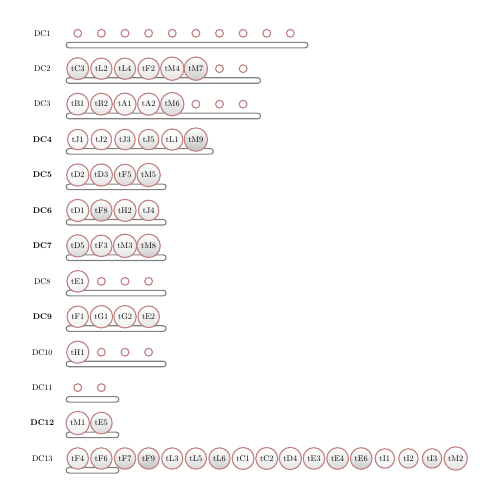
\begin{tikzpicture}[scale=0.3, every node/.style={scale=0.3}]

\tikzstyle{dc} = [rounded rectangle,right,draw=gray,yshift=-0.5cm];
\tikzstyle{task} = [circle,draw=red!50!black!50,top color=white];
\tikzstyle{dp}=[draw,opacity=0.3]
\node at (-1.5,0) {DC1};
\node[dc,text width=10.0cm] (DC1) at (-0.5,0) {};
\node[task] at (0,0) {};
\node[task] at (1,0) {};
\node[task] at (2,0) {};
\node[task] at (3,0) {};
\node[task] at (4,0) {};
\node[task] at (5,0) {};
\node[task] at (6,0) {};
\node[task] at (7,0) {};
\node[task] at (8,0) {};
\node[task] at (9,0) {};
\node at (-1.5,-1.5) {DC2};
\node[dc,text width=8.0cm] (DC2) at (-0.5,-1.5) {};
\node[task,bottom color=black!15.0] at (0,-1.5) {tC3};
\node[task,bottom color=black!10.0] at (1,-1.5) {tL2};
\node[task,bottom color=black!15.0] at (2,-1.5) {tL4};
\node[task,bottom color=black!10.0] at (3,-1.5) {tF2};
\node[task,bottom color=black!10.0] at (4,-1.5) {tM4};
\node[task,bottom color=black!20.0] at (5,-1.5) {tM7};
\node[task] at (6,-1.5) {};
\node[task] at (7,-1.5) {};
\node at (-1.5,-3.0) {DC3};
\node[dc,text width=8.0cm] (DC3) at (-0.5,-3.0) {};
\node[task,bottom color=black!5.0] at (0,-3.0) {tB1};
\node[task,bottom color=black!10.0] at (1,-3.0) {tB2};
\node[task,bottom color=black!5.0] at (2,-3.0) {tA1};
\node[task,bottom color=black!5.0] at (3,-3.0) {tA2};
\node[task,bottom color=black!15.0] at (4,-3.0) {tM6};
\node[task] at (5,-3.0) {};
\node[task] at (6,-3.0) {};
\node[task] at (7,-3.0) {};
\node[font=\bfseries] at (-1.5,-4.5) {DC4};
\node[dc,text width=6.0cm] (DC4) at (-0.5,-4.5) {};
\node[task,bottom color=black!5.0] at (0,-4.5) {tJ1};
\node[task,bottom color=black!5.0] at (1,-4.5) {tJ2};
\node[task,bottom color=black!10.0] at (2,-4.5) {tJ3};
\node[task,bottom color=black!15.0] at (3,-4.5) {tJ5};
\node[task,bottom color=black!5.0] at (4,-4.5) {tL1};
\node[task,bottom color=black!25.0] at (5,-4.5) {tM9};
\node[font=\bfseries] at (-1.5,-6.0) {DC5};
\node[dc,text width=4.0cm] (DC5) at (-0.5,-6.0) {};
\node[task,bottom color=black!5.0] at (0,-6.0) {tD2};
\node[task,bottom color=black!10.0] at (1,-6.0) {tD3};
\node[task,bottom color=black!15.0] at (2,-6.0) {tF5};
\node[task,bottom color=black!15.0] at (3,-6.0) {tM5};
\node[font=\bfseries] at (-1.5,-7.5) {DC6};
\node[dc,text width=4.0cm] (DC6) at (-0.5,-7.5) {};
\node[task,bottom color=black!5.0] at (0,-7.5) {tD1};
\node[task,bottom color=black!20.0] at (1,-7.5) {tF8};
\node[task,bottom color=black!10.0] at (2,-7.5) {tH2};
\node[task,bottom color=black!10.0] at (3,-7.5) {tJ4};
\node[font=\bfseries] at (-1.5,-9.0) {DC7};
\node[dc,text width=4.0cm] (DC7) at (-0.5,-9.0) {};
\node[task,bottom color=black!15.0] at (0,-9.0) {tD5};
\node[task,bottom color=black!10.0] at (1,-9.0) {tF3};
\node[task,bottom color=black!10.0] at (2,-9.0) {tM3};
\node[task,bottom color=black!20.0] at (3,-9.0) {tM8};
\node at (-1.5,-10.5) {DC8};
\node[dc,text width=4.0cm] (DC8) at (-0.5,-10.5) {};
\node[task,bottom color=black!5.0] at (0,-10.5) {tE1};
\node[task] at (1,-10.5) {};
\node[task] at (2,-10.5) {};
\node[task] at (3,-10.5) {};
\node[font=\bfseries] at (-1.5,-12.0) {DC9};
\node[dc,text width=4.0cm] (DC9) at (-0.5,-12.0) {};
\node[task,bottom color=black!5.0] at (0,-12.0) {tF1};
\node[task,bottom color=black!5.0] at (1,-12.0) {tG1};
\node[task,bottom color=black!5.0] at (2,-12.0) {tG2};
\node[task,bottom color=black!10.0] at (3,-12.0) {tE2};
\node at (-1.5,-13.5) {DC10};
\node[dc,text width=4.0cm] (DC10) at (-0.5,-13.5) {};
\node[task,bottom color=black!5.0] at (0,-13.5) {tH1};
\node[task] at (1,-13.5) {};
\node[task] at (2,-13.5) {};
\node[task] at (3,-13.5) {};
\node at (-1.5,-15.0) {DC11};
\node[dc,text width=2.0cm] (DC11) at (-0.5,-15.0) {};
\node[task] at (0,-15.0) {};
\node[task] at (1,-15.0) {};
\node[font=\bfseries] at (-1.5,-16.5) {DC12};
\node[dc,text width=2.0cm] (DC12) at (-0.5,-16.5) {};
\node[task,bottom color=black!5.0] at (0,-16.5) {tM1};
\node[task,bottom color=black!15.0] at (1,-16.5) {tE5};
\node at (-1.5,-18.0) {DC13};
\node[dc,text width=2.0cm] (DC13) at (-0.5,-18.0) {};
\node[task,bottom color=black!10.0] at (0,-18.0) {tF4};
\node[task,bottom color=black!15.0] at (1,-18.0) {tF6};
\node[task,bottom color=black!20.0] at (2,-18.0) {tF7};
\node[task,bottom color=black!25.0] at (3,-18.0) {tF9};
\node[task,bottom color=black!10.0] at (4,-18.0) {tL3};
\node[task,bottom color=black!15.0] at (5,-18.0) {tL5};
\node[task,bottom color=black!20.0] at (6,-18.0) {tL6};
\node[task,bottom color=black!5.0] at (7,-18.0) {tC1};
\node[task,bottom color=black!10.0] at (8,-18.0) {tC2};
\node[task,bottom color=black!10.0] at (9,-18.0) {tD4};
\node[task,bottom color=black!10.0] at (10,-18.0) {tE3};
\node[task,bottom color=black!15.0] at (11,-18.0) {tE4};
\node[task,bottom color=black!20.0] at (12,-18.0) {tE6};
\node[task,bottom color=black!5.0] at (13,-18.0) {tI1};
\node[task,bottom color=black!10.0] at (14,-18.0) {tI2};
\node[task,bottom color=black!15.0] at (15,-18.0) {tI3};
\node[task,bottom color=black!10.0] at (16,-18.0) {tM2};
\end{tikzpicture}
 &  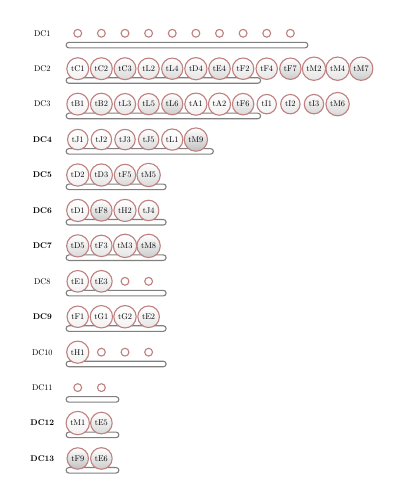
\begin{tikzpicture}[scale=0.3, every node/.style={scale=0.3}]

\tikzstyle{dc} = [rounded rectangle,right,draw=gray,yshift=-0.5cm];
\tikzstyle{task} = [circle,draw=red!50!black!50,top color=white];
\tikzstyle{dp}=[draw,opacity=0.3]
\node at (-1.5,0) {DC1};
\node[dc,text width=10.0cm] (DC1) at (-0.5,0) {};
\node[task] at (0,0) {};
\node[task] at (1,0) {};
\node[task] at (2,0) {};
\node[task] at (3,0) {};
\node[task] at (4,0) {};
\node[task] at (5,0) {};
\node[task] at (6,0) {};
\node[task] at (7,0) {};
\node[task] at (8,0) {};
\node[task] at (9,0) {};
\node at (-1.5,-1.5) {DC2};
\node[dc,text width=8.0cm] (DC2) at (-0.5,-1.5) {};
\node[task,bottom color=black!5.0] at (0,-1.5) {tC1};
\node[task,bottom color=black!10.0] at (1,-1.5) {tC2};
\node[task,bottom color=black!15.0] at (2,-1.5) {tC3};
\node[task,bottom color=black!10.0] at (3,-1.5) {tL2};
\node[task,bottom color=black!15.0] at (4,-1.5) {tL4};
\node[task,bottom color=black!10.0] at (5,-1.5) {tD4};
\node[task,bottom color=black!15.0] at (6,-1.5) {tE4};
\node[task,bottom color=black!10.0] at (7,-1.5) {tF2};
\node[task,bottom color=black!10.0] at (8,-1.5) {tF4};
\node[task,bottom color=black!20.0] at (9,-1.5) {tF7};
\node[task,bottom color=black!10.0] at (10,-1.5) {tM2};
\node[task,bottom color=black!10.0] at (11,-1.5) {tM4};
\node[task,bottom color=black!20.0] at (12,-1.5) {tM7};
\node at (-1.5,-3.0) {DC3};
\node[dc,text width=8.0cm] (DC3) at (-0.5,-3.0) {};
\node[task,bottom color=black!5.0] at (0,-3.0) {tB1};
\node[task,bottom color=black!10.0] at (1,-3.0) {tB2};
\node[task,bottom color=black!10.0] at (2,-3.0) {tL3};
\node[task,bottom color=black!15.0] at (3,-3.0) {tL5};
\node[task,bottom color=black!20.0] at (4,-3.0) {tL6};
\node[task,bottom color=black!5.0] at (5,-3.0) {tA1};
\node[task,bottom color=black!5.0] at (6,-3.0) {tA2};
\node[task,bottom color=black!15.0] at (7,-3.0) {tF6};
\node[task,bottom color=black!5.0] at (8,-3.0) {tI1};
\node[task,bottom color=black!10.0] at (9,-3.0) {tI2};
\node[task,bottom color=black!15.0] at (10,-3.0) {tI3};
\node[task,bottom color=black!15.0] at (11,-3.0) {tM6};
\node[font=\bfseries] at (-1.5,-4.5) {DC4};
\node[dc,text width=6.0cm] (DC4) at (-0.5,-4.5) {};
\node[task,bottom color=black!5.0] at (0,-4.5) {tJ1};
\node[task,bottom color=black!5.0] at (1,-4.5) {tJ2};
\node[task,bottom color=black!10.0] at (2,-4.5) {tJ3};
\node[task,bottom color=black!15.0] at (3,-4.5) {tJ5};
\node[task,bottom color=black!5.0] at (4,-4.5) {tL1};
\node[task,bottom color=black!25.0] at (5,-4.5) {tM9};
\node[font=\bfseries] at (-1.5,-6.0) {DC5};
\node[dc,text width=4.0cm] (DC5) at (-0.5,-6.0) {};
\node[task,bottom color=black!5.0] at (0,-6.0) {tD2};
\node[task,bottom color=black!10.0] at (1,-6.0) {tD3};
\node[task,bottom color=black!15.0] at (2,-6.0) {tF5};
\node[task,bottom color=black!15.0] at (3,-6.0) {tM5};
\node[font=\bfseries] at (-1.5,-7.5) {DC6};
\node[dc,text width=4.0cm] (DC6) at (-0.5,-7.5) {};
\node[task,bottom color=black!5.0] at (0,-7.5) {tD1};
\node[task,bottom color=black!20.0] at (1,-7.5) {tF8};
\node[task,bottom color=black!10.0] at (2,-7.5) {tH2};
\node[task,bottom color=black!10.0] at (3,-7.5) {tJ4};
\node[font=\bfseries] at (-1.5,-9.0) {DC7};
\node[dc,text width=4.0cm] (DC7) at (-0.5,-9.0) {};
\node[task,bottom color=black!15.0] at (0,-9.0) {tD5};
\node[task,bottom color=black!10.0] at (1,-9.0) {tF3};
\node[task,bottom color=black!10.0] at (2,-9.0) {tM3};
\node[task,bottom color=black!20.0] at (3,-9.0) {tM8};
\node at (-1.5,-10.5) {DC8};
\node[dc,text width=4.0cm] (DC8) at (-0.5,-10.5) {};
\node[task,bottom color=black!5.0] at (0,-10.5) {tE1};
\node[task,bottom color=black!10.0] at (1,-10.5) {tE3};
\node[task] at (2,-10.5) {};
\node[task] at (3,-10.5) {};
\node[font=\bfseries] at (-1.5,-12.0) {DC9};
\node[dc,text width=4.0cm] (DC9) at (-0.5,-12.0) {};
\node[task,bottom color=black!5.0] at (0,-12.0) {tF1};
\node[task,bottom color=black!5.0] at (1,-12.0) {tG1};
\node[task,bottom color=black!5.0] at (2,-12.0) {tG2};
\node[task,bottom color=black!10.0] at (3,-12.0) {tE2};
\node at (-1.5,-13.5) {DC10};
\node[dc,text width=4.0cm] (DC10) at (-0.5,-13.5) {};
\node[task,bottom color=black!5.0] at (0,-13.5) {tH1};
\node[task] at (1,-13.5) {};
\node[task] at (2,-13.5) {};
\node[task] at (3,-13.5) {};
\node at (-1.5,-15.0) {DC11};
\node[dc,text width=2.0cm] (DC11) at (-0.5,-15.0) {};
\node[task] at (0,-15.0) {};
\node[task] at (1,-15.0) {};
\node[font=\bfseries] at (-1.5,-16.5) {DC12};
\node[dc,text width=2.0cm] (DC12) at (-0.5,-16.5) {};
\node[task,bottom color=black!5.0] at (0,-16.5) {tM1};
\node[task,bottom color=black!15.0] at (1,-16.5) {tE5};
\node[font=\bfseries] at (-1.5,-18.0) {DC13};
\node[dc,text width=2.0cm] (DC13) at (-0.5,-18.0) {};
\node[task,bottom color=black!25.0] at (0,-18.0) {tF9};
\node[task,bottom color=black!20.0] at (1,-18.0) {tE6};
\end{tikzpicture}
\\
         \hspace*{2em} Iteration 0 & \hspace*{2em} Iteration 1  &\hspace*{2em} Iteration 2 \\
     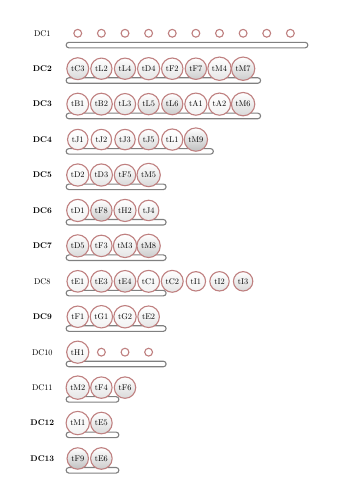
\begin{tikzpicture}[scale=0.3, every node/.style={scale=0.3}]

\tikzstyle{dc} = [rounded rectangle,right,draw=gray,yshift=-0.5cm];
\tikzstyle{task} = [circle,draw=red!50!black!50,top color=white];
\tikzstyle{dp}=[draw,opacity=0.3]
\node at (-1.5,0) {DC1};
\node[dc,text width=10.0cm] (DC1) at (-0.5,0) {};
\node[task] at (0,0) {};
\node[task] at (1,0) {};
\node[task] at (2,0) {};
\node[task] at (3,0) {};
\node[task] at (4,0) {};
\node[task] at (5,0) {};
\node[task] at (6,0) {};
\node[task] at (7,0) {};
\node[task] at (8,0) {};
\node[task] at (9,0) {};
\node[font=\bfseries] at (-1.5,-1.5) {DC2};
\node[dc,text width=8.0cm] (DC2) at (-0.5,-1.5) {};
\node[task,bottom color=black!15.0] at (0,-1.5) {tC3};
\node[task,bottom color=black!10.0] at (1,-1.5) {tL2};
\node[task,bottom color=black!15.0] at (2,-1.5) {tL4};
\node[task,bottom color=black!10.0] at (3,-1.5) {tD4};
\node[task,bottom color=black!10.0] at (4,-1.5) {tF2};
\node[task,bottom color=black!20.0] at (5,-1.5) {tF7};
\node[task,bottom color=black!10.0] at (6,-1.5) {tM4};
\node[task,bottom color=black!20.0] at (7,-1.5) {tM7};
\node[font=\bfseries] at (-1.5,-3.0) {DC3};
\node[dc,text width=8.0cm] (DC3) at (-0.5,-3.0) {};
\node[task,bottom color=black!5.0] at (0,-3.0) {tB1};
\node[task,bottom color=black!10.0] at (1,-3.0) {tB2};
\node[task,bottom color=black!10.0] at (2,-3.0) {tL3};
\node[task,bottom color=black!15.0] at (3,-3.0) {tL5};
\node[task,bottom color=black!20.0] at (4,-3.0) {tL6};
\node[task,bottom color=black!5.0] at (5,-3.0) {tA1};
\node[task,bottom color=black!5.0] at (6,-3.0) {tA2};
\node[task,bottom color=black!15.0] at (7,-3.0) {tM6};
\node[font=\bfseries] at (-1.5,-4.5) {DC4};
\node[dc,text width=6.0cm] (DC4) at (-0.5,-4.5) {};
\node[task,bottom color=black!5.0] at (0,-4.5) {tJ1};
\node[task,bottom color=black!5.0] at (1,-4.5) {tJ2};
\node[task,bottom color=black!10.0] at (2,-4.5) {tJ3};
\node[task,bottom color=black!15.0] at (3,-4.5) {tJ5};
\node[task,bottom color=black!5.0] at (4,-4.5) {tL1};
\node[task,bottom color=black!25.0] at (5,-4.5) {tM9};
\node[font=\bfseries] at (-1.5,-6.0) {DC5};
\node[dc,text width=4.0cm] (DC5) at (-0.5,-6.0) {};
\node[task,bottom color=black!5.0] at (0,-6.0) {tD2};
\node[task,bottom color=black!10.0] at (1,-6.0) {tD3};
\node[task,bottom color=black!15.0] at (2,-6.0) {tF5};
\node[task,bottom color=black!15.0] at (3,-6.0) {tM5};
\node[font=\bfseries] at (-1.5,-7.5) {DC6};
\node[dc,text width=4.0cm] (DC6) at (-0.5,-7.5) {};
\node[task,bottom color=black!5.0] at (0,-7.5) {tD1};
\node[task,bottom color=black!20.0] at (1,-7.5) {tF8};
\node[task,bottom color=black!10.0] at (2,-7.5) {tH2};
\node[task,bottom color=black!10.0] at (3,-7.5) {tJ4};
\node[font=\bfseries] at (-1.5,-9.0) {DC7};
\node[dc,text width=4.0cm] (DC7) at (-0.5,-9.0) {};
\node[task,bottom color=black!15.0] at (0,-9.0) {tD5};
\node[task,bottom color=black!10.0] at (1,-9.0) {tF3};
\node[task,bottom color=black!10.0] at (2,-9.0) {tM3};
\node[task,bottom color=black!20.0] at (3,-9.0) {tM8};
\node at (-1.5,-10.5) {DC8};
\node[dc,text width=4.0cm] (DC8) at (-0.5,-10.5) {};
\node[task,bottom color=black!5.0] at (0,-10.5) {tE1};
\node[task,bottom color=black!10.0] at (1,-10.5) {tE3};
\node[task,bottom color=black!15.0] at (2,-10.5) {tE4};
\node[task,bottom color=black!5.0] at (3,-10.5) {tC1};
\node[task,bottom color=black!10.0] at (4,-10.5) {tC2};
\node[task,bottom color=black!5.0] at (5,-10.5) {tI1};
\node[task,bottom color=black!10.0] at (6,-10.5) {tI2};
\node[task,bottom color=black!15.0] at (7,-10.5) {tI3};
\node[font=\bfseries] at (-1.5,-12.0) {DC9};
\node[dc,text width=4.0cm] (DC9) at (-0.5,-12.0) {};
\node[task,bottom color=black!5.0] at (0,-12.0) {tF1};
\node[task,bottom color=black!5.0] at (1,-12.0) {tG1};
\node[task,bottom color=black!5.0] at (2,-12.0) {tG2};
\node[task,bottom color=black!10.0] at (3,-12.0) {tE2};
\node at (-1.5,-13.5) {DC10};
\node[dc,text width=4.0cm] (DC10) at (-0.5,-13.5) {};
\node[task,bottom color=black!5.0] at (0,-13.5) {tH1};
\node[task] at (1,-13.5) {};
\node[task] at (2,-13.5) {};
\node[task] at (3,-13.5) {};
\node at (-1.5,-15.0) {DC11};
\node[dc,text width=2.0cm] (DC11) at (-0.5,-15.0) {};
\node[task,bottom color=black!10.0] at (0,-15.0) {tM2};
\node[task,bottom color=black!10.0] at (1,-15.0) {tF4};
\node[task,bottom color=black!15.0] at (2,-15.0) {tF6};
\node[font=\bfseries] at (-1.5,-16.5) {DC12};
\node[dc,text width=2.0cm] (DC12) at (-0.5,-16.5) {};
\node[task,bottom color=black!5.0] at (0,-16.5) {tM1};
\node[task,bottom color=black!15.0] at (1,-16.5) {tE5};
\node[font=\bfseries] at (-1.5,-18.0) {DC13};
\node[dc,text width=2.0cm] (DC13) at (-0.5,-18.0) {};
\node[task,bottom color=black!25.0] at (0,-18.0) {tF9};
\node[task,bottom color=black!20.0] at (1,-18.0) {tE6};
\end{tikzpicture}
 & 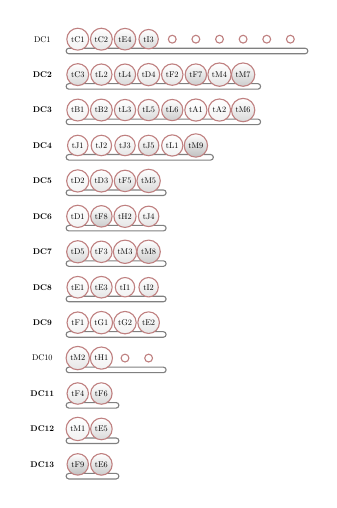
\begin{tikzpicture}[scale=0.3, every node/.style={scale=0.3}]

\tikzstyle{dc} = [rounded rectangle,right,draw=gray,yshift=-0.5cm];
\tikzstyle{task} = [circle,draw=red!50!black!50,top color=white];
\tikzstyle{dp}=[draw,opacity=0.3]
\node at (-1.5,0) {DC1};
\node[dc,text width=10.0cm] (DC1) at (-0.5,0) {};
\node[task,bottom color=black!5.0] at (0,0) {tC1};
\node[task,bottom color=black!10.0] at (1,0) {tC2};
\node[task,bottom color=black!15.0] at (2,0) {tE4};
\node[task,bottom color=black!15.0] at (3,0) {tI3};
\node[task] at (4,0) {};
\node[task] at (5,0) {};
\node[task] at (6,0) {};
\node[task] at (7,0) {};
\node[task] at (8,0) {};
\node[task] at (9,0) {};
\node[font=\bfseries] at (-1.5,-1.5) {DC2};
\node[dc,text width=8.0cm] (DC2) at (-0.5,-1.5) {};
\node[task,bottom color=black!15.0] at (0,-1.5) {tC3};
\node[task,bottom color=black!10.0] at (1,-1.5) {tL2};
\node[task,bottom color=black!15.0] at (2,-1.5) {tL4};
\node[task,bottom color=black!10.0] at (3,-1.5) {tD4};
\node[task,bottom color=black!10.0] at (4,-1.5) {tF2};
\node[task,bottom color=black!20.0] at (5,-1.5) {tF7};
\node[task,bottom color=black!10.0] at (6,-1.5) {tM4};
\node[task,bottom color=black!20.0] at (7,-1.5) {tM7};
\node[font=\bfseries] at (-1.5,-3.0) {DC3};
\node[dc,text width=8.0cm] (DC3) at (-0.5,-3.0) {};
\node[task,bottom color=black!5.0] at (0,-3.0) {tB1};
\node[task,bottom color=black!10.0] at (1,-3.0) {tB2};
\node[task,bottom color=black!10.0] at (2,-3.0) {tL3};
\node[task,bottom color=black!15.0] at (3,-3.0) {tL5};
\node[task,bottom color=black!20.0] at (4,-3.0) {tL6};
\node[task,bottom color=black!5.0] at (5,-3.0) {tA1};
\node[task,bottom color=black!5.0] at (6,-3.0) {tA2};
\node[task,bottom color=black!15.0] at (7,-3.0) {tM6};
\node[font=\bfseries] at (-1.5,-4.5) {DC4};
\node[dc,text width=6.0cm] (DC4) at (-0.5,-4.5) {};
\node[task,bottom color=black!5.0] at (0,-4.5) {tJ1};
\node[task,bottom color=black!5.0] at (1,-4.5) {tJ2};
\node[task,bottom color=black!10.0] at (2,-4.5) {tJ3};
\node[task,bottom color=black!15.0] at (3,-4.5) {tJ5};
\node[task,bottom color=black!5.0] at (4,-4.5) {tL1};
\node[task,bottom color=black!25.0] at (5,-4.5) {tM9};
\node[font=\bfseries] at (-1.5,-6.0) {DC5};
\node[dc,text width=4.0cm] (DC5) at (-0.5,-6.0) {};
\node[task,bottom color=black!5.0] at (0,-6.0) {tD2};
\node[task,bottom color=black!10.0] at (1,-6.0) {tD3};
\node[task,bottom color=black!15.0] at (2,-6.0) {tF5};
\node[task,bottom color=black!15.0] at (3,-6.0) {tM5};
\node[font=\bfseries] at (-1.5,-7.5) {DC6};
\node[dc,text width=4.0cm] (DC6) at (-0.5,-7.5) {};
\node[task,bottom color=black!5.0] at (0,-7.5) {tD1};
\node[task,bottom color=black!20.0] at (1,-7.5) {tF8};
\node[task,bottom color=black!10.0] at (2,-7.5) {tH2};
\node[task,bottom color=black!10.0] at (3,-7.5) {tJ4};
\node[font=\bfseries] at (-1.5,-9.0) {DC7};
\node[dc,text width=4.0cm] (DC7) at (-0.5,-9.0) {};
\node[task,bottom color=black!15.0] at (0,-9.0) {tD5};
\node[task,bottom color=black!10.0] at (1,-9.0) {tF3};
\node[task,bottom color=black!10.0] at (2,-9.0) {tM3};
\node[task,bottom color=black!20.0] at (3,-9.0) {tM8};
\node[font=\bfseries] at (-1.5,-10.5) {DC8};
\node[dc,text width=4.0cm] (DC8) at (-0.5,-10.5) {};
\node[task,bottom color=black!5.0] at (0,-10.5) {tE1};
\node[task,bottom color=black!10.0] at (1,-10.5) {tE3};
\node[task,bottom color=black!5.0] at (2,-10.5) {tI1};
\node[task,bottom color=black!10.0] at (3,-10.5) {tI2};
\node[font=\bfseries] at (-1.5,-12.0) {DC9};
\node[dc,text width=4.0cm] (DC9) at (-0.5,-12.0) {};
\node[task,bottom color=black!5.0] at (0,-12.0) {tF1};
\node[task,bottom color=black!5.0] at (1,-12.0) {tG1};
\node[task,bottom color=black!5.0] at (2,-12.0) {tG2};
\node[task,bottom color=black!10.0] at (3,-12.0) {tE2};
\node at (-1.5,-13.5) {DC10};
\node[dc,text width=4.0cm] (DC10) at (-0.5,-13.5) {};
\node[task,bottom color=black!10.0] at (0,-13.5) {tM2};
\node[task,bottom color=black!5.0] at (1,-13.5) {tH1};
\node[task] at (2,-13.5) {};
\node[task] at (3,-13.5) {};
\node[font=\bfseries] at (-1.5,-15.0) {DC11};
\node[dc,text width=2.0cm] (DC11) at (-0.5,-15.0) {};
\node[task,bottom color=black!10.0] at (0,-15.0) {tF4};
\node[task,bottom color=black!15.0] at (1,-15.0) {tF6};
\node[font=\bfseries] at (-1.5,-16.5) {DC12};
\node[dc,text width=2.0cm] (DC12) at (-0.5,-16.5) {};
\node[task,bottom color=black!5.0] at (0,-16.5) {tM1};
\node[task,bottom color=black!15.0] at (1,-16.5) {tE5};
\node[font=\bfseries] at (-1.5,-18.0) {DC13};
\node[dc,text width=2.0cm] (DC13) at (-0.5,-18.0) {};
\node[task,bottom color=black!25.0] at (0,-18.0) {tF9};
\node[task,bottom color=black!20.0] at (1,-18.0) {tE6};
\end{tikzpicture}
 &
     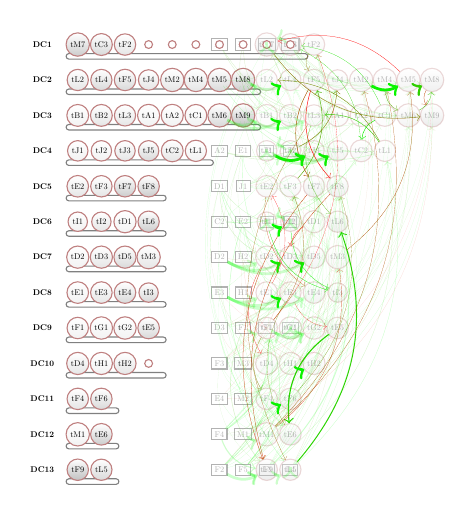
\begin{tikzpicture}[scale=0.3,every node/.style={scale=0.3}]

\tikzstyle{dc} = [rounded rectangle,right,draw=gray,yshift=-0.5cm];
\tikzstyle{task} = [circle,draw=red!50!black!50,top color=white];
\tikzstyle{dp}=[draw,opacity=0.3]
\node[font=\bfseries] at (-1.5,0) {DC1};
\node[dc,text width=10.0cm] (DC1) at (-0.5,0) {};
\node[dp] (A1) at (6,0) {A1};
\node[dp] (B1) at (7,0) {B1};
\node[dp] (M4) at (8,0) {M4};
\node[dp] (M5) at (9,0) {M5};
\node[task,bottom color=black!20.0] at (0,0) {tM7};
\node[task,bottom color=black!20.0,opacity=0.3] (tM7) at (8,0) {tM7};
\node[task,bottom color=black!15.0] at (1,0) {tC3};
\node[task,bottom color=black!15.0,opacity=0.3] (tC3) at (9,0) {tC3};
\node[task,bottom color=black!10.0] at (2,0) {tF2};
\node[task,bottom color=black!10.0,opacity=0.3] (tF2) at (10,0) {tF2};
\node[task] at (3,0) {};
\node[task] at (4,0) {};
\node[task] at (5,0) {};
\node[task] at (6,0) {};
\node[task] at (7,0) {};
\node[task] at (8,0) {};
\node[task] at (9,0) {};
\node[font=\bfseries] at (-1.5,-1.5) {DC2};
\node[dc,text width=8.0cm] (DC2) at (-0.5,-1.5) {};
\node[dp] (C1) at (6,-1.5) {C1};
\node[dp] (L2) at (7,-1.5) {L2};
\node[task,bottom color=black!10.0] at (0,-1.5) {tL2};
\node[task,bottom color=black!10.0,opacity=0.3] (tL2) at (8,-1.5) {tL2};
\node[task,bottom color=black!15.0] at (1,-1.5) {tL4};
\node[task,bottom color=black!15.0,opacity=0.3] (tL4) at (9,-1.5) {tL4};
\node[task,bottom color=black!15.0] at (2,-1.5) {tF5};
\node[task,bottom color=black!15.0,opacity=0.3] (tF5) at (10,-1.5) {tF5};
\node[task,bottom color=black!10.0] at (3,-1.5) {tJ4};
\node[task,bottom color=black!10.0,opacity=0.3] (tJ4) at (11,-1.5) {tJ4};
\node[task,bottom color=black!10.0] at (4,-1.5) {tM2};
\node[task,bottom color=black!10.0,opacity=0.3] (tM2) at (12,-1.5) {tM2};
\node[task,bottom color=black!10.0] at (5,-1.5) {tM4};
\node[task,bottom color=black!10.0,opacity=0.3] (tM4) at (13,-1.5) {tM4};
\node[task,bottom color=black!15.0] at (6,-1.5) {tM5};
\node[task,bottom color=black!15.0,opacity=0.3] (tM5) at (14,-1.5) {tM5};
\node[task,bottom color=black!20.0] at (7,-1.5) {tM8};
\node[task,bottom color=black!20.0,opacity=0.3] (tM8) at (15,-1.5) {tM8};
\node[font=\bfseries] at (-1.5,-3.0) {DC3};
\node[dc,text width=8.0cm] (DC3) at (-0.5,-3.0) {};
\node[dp] (B2) at (6,-3.0) {B2};
\node[dp] (L1) at (7,-3.0) {L1};
\node[task,bottom color=black!5.0] at (0,-3.0) {tB1};
\node[task,bottom color=black!5.0,opacity=0.3] (tB1) at (8,-3.0) {tB1};
\node[task,bottom color=black!10.0] at (1,-3.0) {tB2};
\node[task,bottom color=black!10.0,opacity=0.3] (tB2) at (9,-3.0) {tB2};
\node[task,bottom color=black!10.0] at (2,-3.0) {tL3};
\node[task,bottom color=black!10.0,opacity=0.3] (tL3) at (10,-3.0) {tL3};
\node[task,bottom color=black!5.0] at (3,-3.0) {tA1};
\node[task,bottom color=black!5.0,opacity=0.3] (tA1) at (11,-3.0) {tA1};
\node[task,bottom color=black!5.0] at (4,-3.0) {tA2};
\node[task,bottom color=black!5.0,opacity=0.3] (tA2) at (12,-3.0) {tA2};
\node[task,bottom color=black!5.0] at (5,-3.0) {tC1};
\node[task,bottom color=black!5.0,opacity=0.3] (tC1) at (13,-3.0) {tC1};
\node[task,bottom color=black!15.0] at (6,-3.0) {tM6};
\node[task,bottom color=black!15.0,opacity=0.3] (tM6) at (14,-3.0) {tM6};
\node[task,bottom color=black!25.0] at (7,-3.0) {tM9};
\node[task,bottom color=black!25.0,opacity=0.3] (tM9) at (15,-3.0) {tM9};
\node[font=\bfseries] at (-1.5,-4.5) {DC4};
\node[dc,text width=6.0cm] (DC4) at (-0.5,-4.5) {};
\node[dp] (A2) at (6,-4.5) {A2};
\node[dp] (E1) at (7,-4.5) {E1};
\node[dp] (J2) at (8,-4.5) {J2};
\node[dp] (J3) at (9,-4.5) {J3};
\node[task,bottom color=black!5.0] at (0,-4.5) {tJ1};
\node[task,bottom color=black!5.0,opacity=0.3] (tJ1) at (8,-4.5) {tJ1};
\node[task,bottom color=black!5.0] at (1,-4.5) {tJ2};
\node[task,bottom color=black!5.0,opacity=0.3] (tJ2) at (9,-4.5) {tJ2};
\node[task,bottom color=black!10.0] at (2,-4.5) {tJ3};
\node[task,bottom color=black!10.0,opacity=0.3] (tJ3) at (10,-4.5) {tJ3};
\node[task,bottom color=black!15.0] at (3,-4.5) {tJ5};
\node[task,bottom color=black!15.0,opacity=0.3] (tJ5) at (11,-4.5) {tJ5};
\node[task,bottom color=black!10.0] at (4,-4.5) {tC2};
\node[task,bottom color=black!10.0,opacity=0.3] (tC2) at (12,-4.5) {tC2};
\node[task,bottom color=black!5.0] at (5,-4.5) {tL1};
\node[task,bottom color=black!5.0,opacity=0.3] (tL1) at (13,-4.5) {tL1};
\node[font=\bfseries] at (-1.5,-6.0) {DC5};
\node[dc,text width=4.0cm] (DC5) at (-0.5,-6.0) {};
\node[dp] (D1) at (6,-6.0) {D1};
\node[dp] (J1) at (7,-6.0) {J1};
\node[task,bottom color=black!10.0] at (0,-6.0) {tE2};
\node[task,bottom color=black!10.0,opacity=0.3] (tE2) at (8,-6.0) {tE2};
\node[task,bottom color=black!10.0] at (1,-6.0) {tF3};
\node[task,bottom color=black!10.0,opacity=0.3] (tF3) at (9,-6.0) {tF3};
\node[task,bottom color=black!20.0] at (2,-6.0) {tF7};
\node[task,bottom color=black!20.0,opacity=0.3] (tF7) at (10,-6.0) {tF7};
\node[task,bottom color=black!20.0] at (3,-6.0) {tF8};
\node[task,bottom color=black!20.0,opacity=0.3] (tF8) at (11,-6.0) {tF8};
\node[font=\bfseries] at (-1.5,-7.5) {DC6};
\node[dc,text width=4.0cm] (DC6) at (-0.5,-7.5) {};
\node[dp] (C2) at (6,-7.5) {C2};
\node[dp] (E2) at (7,-7.5) {E2};
\node[dp] (I1) at (8,-7.5) {I1};
\node[dp] (I2) at (9,-7.5) {I2};
\node[task,bottom color=black!5.0] at (0,-7.5) {tI1};
\node[task,bottom color=black!5.0,opacity=0.3] (tI1) at (8,-7.5) {tI1};
\node[task,bottom color=black!10.0] at (1,-7.5) {tI2};
\node[task,bottom color=black!10.0,opacity=0.3] (tI2) at (9,-7.5) {tI2};
\node[task,bottom color=black!5.0] at (2,-7.5) {tD1};
\node[task,bottom color=black!5.0,opacity=0.3] (tD1) at (10,-7.5) {tD1};
\node[task,bottom color=black!20.0] at (3,-7.5) {tL6};
\node[task,bottom color=black!20.0,opacity=0.3] (tL6) at (11,-7.5) {tL6};
\node[font=\bfseries] at (-1.5,-9.0) {DC7};
\node[dc,text width=4.0cm] (DC7) at (-0.5,-9.0) {};
\node[dp] (D2) at (6,-9.0) {D2};
\node[dp] (H2) at (7,-9.0) {H2};
\node[task,bottom color=black!5.0] at (0,-9.0) {tD2};
\node[task,bottom color=black!5.0,opacity=0.3] (tD2) at (8,-9.0) {tD2};
\node[task,bottom color=black!10.0] at (1,-9.0) {tD3};
\node[task,bottom color=black!10.0,opacity=0.3] (tD3) at (9,-9.0) {tD3};
\node[task,bottom color=black!15.0] at (2,-9.0) {tD5};
\node[task,bottom color=black!15.0,opacity=0.3] (tD5) at (10,-9.0) {tD5};
\node[task,bottom color=black!10.0] at (3,-9.0) {tM3};
\node[task,bottom color=black!10.0,opacity=0.3] (tM3) at (11,-9.0) {tM3};
\node[font=\bfseries] at (-1.5,-10.5) {DC8};
\node[dc,text width=4.0cm] (DC8) at (-0.5,-10.5) {};
\node[dp] (E3) at (6,-10.5) {E3};
\node[dp] (H1) at (7,-10.5) {H1};
\node[task,bottom color=black!5.0] at (0,-10.5) {tE1};
\node[task,bottom color=black!5.0,opacity=0.3] (tE1) at (8,-10.5) {tE1};
\node[task,bottom color=black!10.0] at (1,-10.5) {tE3};
\node[task,bottom color=black!10.0,opacity=0.3] (tE3) at (9,-10.5) {tE3};
\node[task,bottom color=black!15.0] at (2,-10.5) {tE4};
\node[task,bottom color=black!15.0,opacity=0.3] (tE4) at (10,-10.5) {tE4};
\node[task,bottom color=black!15.0] at (3,-10.5) {tI3};
\node[task,bottom color=black!15.0,opacity=0.3] (tI3) at (11,-10.5) {tI3};
\node[font=\bfseries] at (-1.5,-12.0) {DC9};
\node[dc,text width=4.0cm] (DC9) at (-0.5,-12.0) {};
\node[dp] (D3) at (6,-12.0) {D3};
\node[dp] (F1) at (7,-12.0) {F1};
\node[dp] (G1) at (8,-12.0) {G1};
\node[dp] (G2) at (9,-12.0) {G2};
\node[task,bottom color=black!5.0] at (0,-12.0) {tF1};
\node[task,bottom color=black!5.0,opacity=0.3] (tF1) at (8,-12.0) {tF1};
\node[task,bottom color=black!5.0] at (1,-12.0) {tG1};
\node[task,bottom color=black!5.0,opacity=0.3] (tG1) at (9,-12.0) {tG1};
\node[task,bottom color=black!5.0] at (2,-12.0) {tG2};
\node[task,bottom color=black!5.0,opacity=0.3] (tG2) at (10,-12.0) {tG2};
\node[task,bottom color=black!15.0] at (3,-12.0) {tE5};
\node[task,bottom color=black!15.0,opacity=0.3] (tE5) at (11,-12.0) {tE5};
\node[font=\bfseries] at (-1.5,-13.5) {DC10};
\node[dc,text width=4.0cm] (DC10) at (-0.5,-13.5) {};
\node[dp] (F3) at (6,-13.5) {F3};
\node[dp] (M3) at (7,-13.5) {M3};
\node[task,bottom color=black!10.0] at (0,-13.5) {tD4};
\node[task,bottom color=black!10.0,opacity=0.3] (tD4) at (8,-13.5) {tD4};
\node[task,bottom color=black!5.0] at (1,-13.5) {tH1};
\node[task,bottom color=black!5.0,opacity=0.3] (tH1) at (9,-13.5) {tH1};
\node[task,bottom color=black!10.0] at (2,-13.5) {tH2};
\node[task,bottom color=black!10.0,opacity=0.3] (tH2) at (10,-13.5) {tH2};
\node[task] at (3,-13.5) {};
\node[font=\bfseries] at (-1.5,-15.0) {DC11};
\node[dc,text width=2.0cm] (DC11) at (-0.5,-15.0) {};
\node[dp] (E4) at (6,-15.0) {E4};
\node[dp] (M2) at (7,-15.0) {M2};
\node[task,bottom color=black!10.0] at (0,-15.0) {tF4};
\node[task,bottom color=black!10.0,opacity=0.3] (tF4) at (8,-15.0) {tF4};
\node[task,bottom color=black!15.0] at (1,-15.0) {tF6};
\node[task,bottom color=black!15.0,opacity=0.3] (tF6) at (9,-15.0) {tF6};
\node[font=\bfseries] at (-1.5,-16.5) {DC12};
\node[dc,text width=2.0cm] (DC12) at (-0.5,-16.5) {};
\node[dp] (F4) at (6,-16.5) {F4};
\node[dp] (M1) at (7,-16.5) {M1};
\node[task,bottom color=black!5.0] at (0,-16.5) {tM1};
\node[task,bottom color=black!5.0,opacity=0.3] (tM1) at (8,-16.5) {tM1};
\node[task,bottom color=black!20.0] at (1,-16.5) {tE6};
\node[task,bottom color=black!20.0,opacity=0.3] (tE6) at (9,-16.5) {tE6};
\node[font=\bfseries] at (-1.5,-18.0) {DC13};
\node[dc,text width=2.0cm] (DC13) at (-0.5,-18.0) {};
\node[dp] (F2) at (6,-18.0) {F2};
\node[dp] (F5) at (7,-18.0) {F5};
\node[dp] (L3) at (8,-18.0) {L3};
\node[dp] (L4) at (9,-18.0) {L4};
\node[task,bottom color=black!25.0] at (0,-18.0) {tF9};
\node[task,bottom color=black!25.0,opacity=0.3] (tF9) at (8,-18.0) {tF9};
\node[task,bottom color=black!15.0] at (1,-18.0) {tL5};
\node[task,bottom color=black!15.0,opacity=0.3] (tL5) at (9,-18.0) {tL5};
\draw[red!3.75!green,line width=1.0pt] (tB1) edge[->,bend right] (tB2);
\draw[red!6.75!green,line width=0.16666666666666666pt] (tC1) edge[->,bend right] (tC2);
\draw[red!11.25!green,line width=0.06666666666666667pt] (tC1) edge[->,bend right] (tC3);
\draw[red!15.0!green,line width=0.05pt] (tC2) edge[->,bend right] (tC3);
\draw[red!95.0!green,line width=0.07894736842105263pt] (tD1) edge[->,bend right] (tD3);
\draw[red!7.5!green,line width=1.0pt] (tD2) edge[->,bend right] (tD3);
\draw[red!100!green,line width=0.058333333333333334pt] (tD2) edge[->,bend right] (tD4);
\draw[red!7.5!green,line width=1.0pt] (tD3) edge[->,bend right] (tD5);
\draw[red!100.0!green,line width=0.0375pt] (tE1) edge[->,bend right] (tE2);
\draw[red!3.0!green,line width=1.0pt] (tE1) edge[->,bend right] (tE3);
\draw[red!80.0!green,line width=0.046875pt] (tE2) edge[->,bend right] (tE4);
\draw[red!93.825!green,line width=0.03597122302158273pt] (tE3) edge[->,bend right] (tE5);
\draw[red!46.49999999999999!green,line width=0.040322580645161296pt] (tE3) edge[->,bend right] (tE6);
\draw[red!16.2!green,line width=0.4166666666666667pt] (tE5) edge[->,bend right] (tE6);
\draw[red!100!green,line width=0.030800821355236138pt] (tF1) edge[->,bend right] (tF2);
\draw[red!65.1!green,line width=0.06912442396313365pt] (tF1) edge[->,bend right] (tF3);
\draw[red!50.0!green,line width=0.075pt] (tF1) edge[->,bend right] (tF4);
\draw[red!56.25!green,line width=0.06666666666666667pt] (tF2) edge[->,bend right] (tF5);
\draw[red!33.75!green,line width=0.16666666666666666pt] (tF3) edge[->,bend right] (tF5);
\draw[red!3.375!green,line width=1.0pt] (tF4) edge[->,bend right] (tF6);
\draw[red!67.5!green,line width=0.16666666666666666pt] (tF5) edge[->,bend right] (tF7);
\draw[red!100!green,line width=0.16666666666666666pt] (tF5) edge[->,bend right] (tF8);
\draw[red!48.75!green,line width=0.038461538461538464pt] (tF6) edge[->,bend right] (tF8);
\draw[red!78.0!green,line width=0.09615384615384616pt] (tF7) edge[->,bend right] (tF9);
\draw[red!78.0!green,line width=0.09615384615384616pt] (tF8) edge[->,bend right] (tF9);
\draw[red!3.75!green,line width=1.0pt] (tH1) edge[->,bend right] (tH2);
\draw[red!1.125!green,line width=1.0pt] (tI1) edge[->,bend right] (tI2);
\draw[red!10.0!green,line width=0.075pt] (tI1) edge[->,bend right] (tI3);
\draw[red!10.0!green,line width=0.075pt] (tI2) edge[->,bend right] (tI3);
\draw[red!7.5!green,line width=1.0pt] (tJ1) edge[->,bend right] (tJ3);
\draw[red!7.5!green,line width=1.0pt] (tJ2) edge[->,bend right] (tJ3);
\draw[red!60.0!green,line width=0.125pt] (tJ2) edge[->,bend right] (tJ4);
\draw[red!7.5!green,line width=1.0pt] (tJ3) edge[->,bend right] (tJ5);
\draw[red!45.0!green,line width=0.125pt] (tL1) edge[->,bend right] (tL2);
\draw[red!20.0!green,line width=0.15pt] (tL1) edge[->,bend right] (tL3);
\draw[red!3.75!green,line width=1.0pt] (tL2) edge[->,bend right] (tL4);
\draw[red!62.099999999999994!green,line width=0.05434782608695652pt] (tL3) edge[->,bend right] (tL5);
\draw[red!30.0!green,line width=0.0625pt] (tL3) edge[->,bend right] (tL6);
\draw[red!20.25!green,line width=0.3333333333333333pt] (tL5) edge[->,bend right] (tL6);
\draw[red!67.75000000000001!green,line width=0.05535055350553505pt] (tM1) edge[->,bend right] (tM2);
\draw[red!81.30000000000001!green,line width=0.05535055350553505pt] (tM1) edge[->,bend right] (tM3);
\draw[red!67.75000000000001!green,line width=0.05535055350553505pt] (tM1) edge[->,bend right] (tM4);
\draw[red!3.75!green,line width=1.0pt] (tM2) edge[->,bend right] (tM5);
\draw[red!67.5!green,line width=0.08333333333333333pt] (tM3) edge[->,bend right] (tM5);
\draw[red!33.75!green,line width=0.1pt] (tM4) edge[->,bend right] (tM6);
\draw[red!100!green,line width=0.08333333333333333pt] (tM5) edge[->,bend right] (tM7);
\draw[red!18.75!green,line width=1.0pt] (tM5) edge[->,bend right] (tM8);
\draw[red!22.5!green,line width=0.08333333333333333pt] (tM6) edge[->,bend right] (tM8);
\draw[red!60.0!green,line width=0.125pt] (tM7) edge[->,bend right] (tM9);
\draw[red!75.0!green,line width=0.1pt] (tM8) edge[->,bend right] (tM9);
\draw[opacity=0.2,red!25.0!green,line width=0.125pt] (A1) edge[->,bend right] (tA1);
\draw[opacity=0.2,red!25.0!green,line width=0.15pt] (A2) edge[->,bend right] (tA1);
\draw[opacity=0.2,red!25.0!green,line width=0.125pt] (A1) edge[->,bend right] (tA2);
\draw[opacity=0.2,red!25.0!green,line width=0.15pt] (A2) edge[->,bend right] (tA2);
\draw[opacity=0.2,red!30.0!green,line width=0.125pt] (B1) edge[->,bend right] (tB1);
\draw[opacity=0.2,red!3.75!green,line width=1.0pt] (B2) edge[->,bend right] (tB1);
\draw[opacity=0.2,red!33.33333333333333!green,line width=0.125pt] (B1) edge[->,bend right] (tB2);
\draw[opacity=0.2,red!6.25!green,line width=1.0pt] (B2) edge[->,bend right] (tB2);
\draw[opacity=0.2,red!10.416666666666668!green,line width=0.1pt] (C1) edge[->,bend right] (tC1);
\draw[opacity=0.2,red!11.944444444444445!green,line width=0.08720930232558138pt] (C2) edge[->,bend right] (tC1);
\draw[opacity=0.2,red!0.0!green,line width=0.13333333333333333pt] (C1) edge[->,bend right] (tC2);
\draw[opacity=0.2,red!7.000000000000001!green,line width=0.20833333333333334pt] (C2) edge[->,bend right] (tC2);
\draw[opacity=0.2,red!7.5!green,line width=0.08333333333333333pt] (C1) edge[->,bend right] (tC3);
\draw[opacity=0.2,red!0.0!green,line width=0.040540540540540536pt] (C2) edge[->,bend right] (tC3);
\draw[opacity=0.2,red!16.666666666666664!green,line width=0.125pt] (D1) edge[->,bend right] (tD1);
\draw[opacity=0.2,red!58.333333333333336!green,line width=0.07142857142857142pt] (D2) edge[->,bend right] (tD1);
\draw[opacity=0.2,red!48.75000000000001!green,line width=0.1282051282051282pt] (D3) edge[->,bend right] (tD1);
\draw[opacity=0.2,red!25.0!green,line width=0.16666666666666666pt] (D1) edge[->,bend right] (tD2);
\draw[opacity=0.2,red!6.25!green,line width=1.0pt] (D2) edge[->,bend right] (tD2);
\draw[opacity=0.2,red!42.63888888888889!green,line width=0.048859934853420196pt] (D3) edge[->,bend right] (tD2);
\draw[opacity=0.2,red!0.0!green,line width=0.16666666666666666pt] (D1) edge[->,bend right] (tD3);
\draw[opacity=0.2,red!1.0416666666666665!green,line width=1.0pt] (D2) edge[->,bend right] (tD3);
\draw[opacity=0.2,red!0.0!green,line width=0.048859934853420196pt] (D3) edge[->,bend right] (tD3);
\draw[opacity=0.2,red!48.21428571428571!green,line width=0.04320987654320988pt] (D1) edge[->,bend right] (tD4);
\draw[opacity=0.2,red!0.0!green,line width=0.058333333333333334pt] (D2) edge[->,bend right] (tD4);
\draw[opacity=0.2,red!71.80555555555556!green,line width=0.029013539651837526pt] (D3) edge[->,bend right] (tD4);
\draw[opacity=0.2,red!0.0!green,line width=0.16666666666666666pt] (D1) edge[->,bend right] (tD5);
\draw[opacity=0.2,red!4.166666666666666!green,line width=1.0pt] (D2) edge[->,bend right] (tD5);
\draw[opacity=0.2,red!0.0!green,line width=0.048859934853420196pt] (D3) edge[->,bend right] (tD5);
\draw[opacity=0.2,red!29.166666666666664!green,line width=0.04285714285714286pt] (E1) edge[->,bend right] (tE1);
\draw[opacity=0.2,red!22.22222222222222!green,line width=0.075pt] (E2) edge[->,bend right] (tE1);
\draw[opacity=0.2,red!2.5!green,line width=1.0pt] (E3) edge[->,bend right] (tE1);
\draw[opacity=0.2,red!0.0!green,line width=0.023076923076923075pt] (E4) edge[->,bend right] (tE1);
\draw[opacity=0.2,red!0.0!green,line width=0.07142857142857142pt] (E1) edge[->,bend right] (tE2);
\draw[opacity=0.2,red!12.5!green,line width=0.15pt] (E2) edge[->,bend right] (tE2);
\draw[opacity=0.2,red!0.0!green,line width=0.0375pt] (E3) edge[->,bend right] (tE2);
\draw[opacity=0.2,red!65.0!green,line width=0.038461538461538464pt] (E4) edge[->,bend right] (tE2);
\draw[opacity=0.2,red!14.583333333333332!green,line width=0.04285714285714286pt] (E1) edge[->,bend right] (tE3);
\draw[opacity=0.2,red!0.0!green,line width=0.075pt] (E2) edge[->,bend right] (tE3);
\draw[opacity=0.2,red!1.0416666666666665!green,line width=1.0pt] (E3) edge[->,bend right] (tE3);
\draw[opacity=0.2,red!0.0!green,line width=0.023076923076923075pt] (E4) edge[->,bend right] (tE3);
\draw[opacity=0.2,red!0.0!green,line width=0.04285714285714286pt] (E1) edge[->,bend right] (tE4);
\draw[opacity=0.2,red!44.44444444444444!green,line width=0.075pt] (E2) edge[->,bend right] (tE4);
\draw[opacity=0.2,red!0.0!green,line width=1.0pt] (E3) edge[->,bend right] (tE4);
\draw[opacity=0.2,red!0.0!green,line width=0.023076923076923075pt] (E4) edge[->,bend right] (tE4);
\draw[opacity=0.2,red!0.0!green,line width=0.05617977528089888pt] (E1) edge[->,bend right] (tE5);
\draw[opacity=0.2,red!0.0!green,line width=0.1282051282051282pt] (E2) edge[->,bend right] (tE5);
\draw[opacity=0.2,red!92.66666666666666!green,line width=0.03597122302158273pt] (E3) edge[->,bend right] (tE5);
\draw[opacity=0.2,red!90.0!green,line width=0.041666666666666664pt] (E4) edge[->,bend right] (tE5);
\draw[opacity=0.2,red!15.416666666666668!green,line width=0.06756756756756757pt] (E1) edge[->,bend right] (tE6);
\draw[opacity=0.2,red!0.0!green,line width=0.20833333333333334pt] (E2) edge[->,bend right] (tE6);
\draw[opacity=0.2,red!0.0!green,line width=0.040322580645161296pt] (E3) edge[->,bend right] (tE6);
\draw[opacity=0.2,red!0.0!green,line width=0.03787878787878789pt] (E4) edge[->,bend right] (tE6);
\draw[opacity=0.2,red!6.25!green,line width=1.0pt] (F1) edge[->,bend right] (tF1);
\draw[opacity=0.2,red!0.0!green,line width=0.18518518518518517pt] (F2) edge[->,bend right] (tF1);
\draw[opacity=0.2,red!0.0!green,line width=0.025678650036683785pt] (F3) edge[->,bend right] (tF1);
\draw[opacity=0.2,red!0.0!green,line width=0.3333333333333333pt] (F4) edge[->,bend right] (tF1);
\draw[opacity=0.2,red!0.0!green,line width=0.18518518518518517pt] (F5) edge[->,bend right] (tF1);
\draw[opacity=0.2,red!0.0!green,line width=0.030800821355236138pt] (F1) edge[->,bend right] (tF2);
\draw[opacity=0.2,red!57.63888888888889!green,line width=0.03614457831325301pt] (F2) edge[->,bend right] (tF2);
\draw[opacity=0.2,red!0.0!green,line width=0.024305555555555552pt] (F3) edge[->,bend right] (tF2);
\draw[opacity=0.2,red!0.0!green,line width=0.03325942350332595pt] (F4) edge[->,bend right] (tF2);
\draw[opacity=0.2,red!0.0!green,line width=0.03614457831325301pt] (F5) edge[->,bend right] (tF2);
\draw[opacity=0.2,red!0.0!green,line width=0.06912442396313365pt] (F1) edge[->,bend right] (tF3);
\draw[opacity=0.2,red!0.0!green,line width=0.10344827586206896pt] (F2) edge[->,bend right] (tF3);
\draw[opacity=0.2,red!96.42857142857142!green,line width=0.04320987654320988pt] (F3) edge[->,bend right] (tF3);
\draw[opacity=0.2,red!0.0!green,line width=0.08287292817679558pt] (F4) edge[->,bend right] (tF3);
\draw[opacity=0.2,red!0.0!green,line width=0.10344827586206896pt] (F5) edge[->,bend right] (tF3);
\draw[opacity=0.2,red!0.0!green,line width=0.075pt] (F1) edge[->,bend right] (tF4);
\draw[opacity=0.2,red!0.0!green,line width=0.05338078291814946pt] (F2) edge[->,bend right] (tF4);
\draw[opacity=0.2,red!0.0!green,line width=0.021212121212121213pt] (F3) edge[->,bend right] (tF4);
\draw[opacity=0.2,red!34.02777777777778!green,line width=0.06122448979591836pt] (F4) edge[->,bend right] (tF4);
\draw[opacity=0.2,red!0.0!green,line width=0.05338078291814946pt] (F5) edge[->,bend right] (tF4);
\draw[opacity=0.2,red!21.319444444444446!green,line width=0.048859934853420196pt] (F1) edge[->,bend right] (tF5);
\draw[opacity=0.2,red!16.319444444444446!green,line width=0.06382978723404255pt] (F2) edge[->,bend right] (tF5);
\draw[opacity=0.2,red!30.357142857142854!green,line width=0.03431372549019608pt] (F3) edge[->,bend right] (tF5);
\draw[opacity=0.2,red!0.0!green,line width=0.05535055350553505pt] (F4) edge[->,bend right] (tF5);
\draw[opacity=0.2,red!0.0!green,line width=0.06382978723404255pt] (F5) edge[->,bend right] (tF5);
\draw[opacity=0.2,red!19.444444444444446!green,line width=0.075pt] (F1) edge[->,bend right] (tF6);
\draw[opacity=0.2,red!0.0!green,line width=0.05338078291814946pt] (F2) edge[->,bend right] (tF6);
\draw[opacity=0.2,red!0.0!green,line width=0.021212121212121213pt] (F3) edge[->,bend right] (tF6);
\draw[opacity=0.2,red!23.819444444444446!green,line width=0.06122448979591836pt] (F4) edge[->,bend right] (tF6);
\draw[opacity=0.2,red!0.0!green,line width=0.05338078291814946pt] (F5) edge[->,bend right] (tF6);
\draw[opacity=0.2,red!0.0!green,line width=0.06912442396313365pt] (F1) edge[->,bend right] (tF7);
\draw[opacity=0.2,red!0.0!green,line width=0.10344827586206896pt] (F2) edge[->,bend right] (tF7);
\draw[opacity=0.2,red!48.21428571428571!green,line width=0.04320987654320988pt] (F3) edge[->,bend right] (tF7);
\draw[opacity=0.2,red!0.0!green,line width=0.08287292817679558pt] (F4) edge[->,bend right] (tF7);
\draw[opacity=0.2,red!40.27777777777778!green,line width=0.10344827586206896pt] (F5) edge[->,bend right] (tF7);
\draw[opacity=0.2,red!0.0!green,line width=0.06912442396313365pt] (F1) edge[->,bend right] (tF8);
\draw[opacity=0.2,red!30.208333333333332!green,line width=0.10344827586206896pt] (F2) edge[->,bend right] (tF8);
\draw[opacity=0.2,red!0.0!green,line width=0.04320987654320988pt] (F3) edge[->,bend right] (tF8);
\draw[opacity=0.2,red!0.0!green,line width=0.08287292817679558pt] (F4) edge[->,bend right] (tF8);
\draw[opacity=0.2,red!20.13888888888889!green,line width=0.10344827586206896pt] (F5) edge[->,bend right] (tF8);
\draw[opacity=0.2,red!25.0!green,line width=0.20833333333333334pt] (F1) edge[->,bend right] (tF9);
\draw[opacity=0.2,red!0.0!green,line width=1.0pt] (F2) edge[->,bend right] (tF9);
\draw[opacity=0.2,red!20.96428571428571!green,line width=0.02981260647359455pt] (F3) edge[->,bend right] (tF9);
\draw[opacity=0.2,red!4.0!green,line width=0.4166666666666667pt] (F4) edge[->,bend right] (tF9);
\draw[opacity=0.2,red!4.166666666666666!green,line width=1.0pt] (F5) edge[->,bend right] (tF9);
\draw[opacity=0.2,red!3.125!green,line width=1.0pt] (G1) edge[->,bend right] (tG1);
\draw[opacity=0.2,red!3.75!green,line width=1.0pt] (G2) edge[->,bend right] (tG1);
\draw[opacity=0.2,red!3.125!green,line width=1.0pt] (G1) edge[->,bend right] (tG2);
\draw[opacity=0.2,red!3.75!green,line width=1.0pt] (G2) edge[->,bend right] (tG2);
\draw[opacity=0.2,red!50.0!green,line width=0.075pt] (H1) edge[->,bend right] (tH1);
\draw[opacity=0.2,red!64.28571428571429!green,line width=0.058333333333333334pt] (H2) edge[->,bend right] (tH1);
\draw[opacity=0.2,red!55.55555555555556!green,line width=0.075pt] (H1) edge[->,bend right] (tH2);
\draw[opacity=0.2,red!100!green,line width=0.058333333333333334pt] (H2) edge[->,bend right] (tH2);
\draw[opacity=0.2,red!1.0416666666666665!green,line width=1.0pt] (I1) edge[->,bend right] (tI1);
\draw[opacity=0.2,red!1.0416666666666665!green,line width=1.0pt] (I2) edge[->,bend right] (tI1);
\draw[opacity=0.2,red!0.0!green,line width=1.0pt] (I1) edge[->,bend right] (tI2);
\draw[opacity=0.2,red!1.4583333333333333!green,line width=1.0pt] (I2) edge[->,bend right] (tI2);
\draw[opacity=0.2,red!8.333333333333332!green,line width=0.075pt] (I1) edge[->,bend right] (tI3);
\draw[opacity=0.2,red!0.0!green,line width=0.075pt] (I2) edge[->,bend right] (tI3);
\draw[opacity=0.2,red!26.66666666666667!green,line width=0.07812499999999999pt] (J1) edge[->,bend right] (tJ1);
\draw[opacity=0.2,red!4.166666666666666!green,line width=1.0pt] (J2) edge[->,bend right] (tJ1);
\draw[opacity=0.2,red!6.25!green,line width=1.0pt] (J3) edge[->,bend right] (tJ1);
\draw[opacity=0.2,red!53.33333333333334!green,line width=0.07812499999999999pt] (J1) edge[->,bend right] (tJ2);
\draw[opacity=0.2,red!6.25!green,line width=1.0pt] (J2) edge[->,bend right] (tJ2);
\draw[opacity=0.2,red!2.083333333333333!green,line width=1.0pt] (J3) edge[->,bend right] (tJ2);
\draw[opacity=0.2,red!0.0!green,line width=0.07812499999999999pt] (J1) edge[->,bend right] (tJ3);
\draw[opacity=0.2,red!1.0416666666666665!green,line width=1.0pt] (J2) edge[->,bend right] (tJ3);
\draw[opacity=0.2,red!0.0!green,line width=1.0pt] (J3) edge[->,bend right] (tJ3);
\draw[opacity=0.2,red!12.5!green,line width=0.16666666666666666pt] (J1) edge[->,bend right] (tJ4);
\draw[opacity=0.2,red!0.0!green,line width=0.125pt] (J2) edge[->,bend right] (tJ4);
\draw[opacity=0.2,red!16.666666666666664!green,line width=0.125pt] (J3) edge[->,bend right] (tJ4);
\draw[opacity=0.2,red!0.0!green,line width=0.07812499999999999pt] (J1) edge[->,bend right] (tJ5);
\draw[opacity=0.2,red!4.166666666666666!green,line width=1.0pt] (J2) edge[->,bend right] (tJ5);
\draw[opacity=0.2,red!0.0!green,line width=1.0pt] (J3) edge[->,bend right] (tJ5);
\draw[opacity=0.2,red!7.5!green,line width=0.16666666666666666pt] (L1) edge[->,bend right] (tL1);
\draw[opacity=0.2,red!12.5!green,line width=0.13333333333333333pt] (L2) edge[->,bend right] (tL1);
\draw[opacity=0.2,red!19.5!green,line width=0.1282051282051282pt] (L3) edge[->,bend right] (tL1);
\draw[opacity=0.2,red!0.0!green,line width=0.1282051282051282pt] (L4) edge[->,bend right] (tL1);
\draw[opacity=0.2,red!0.0!green,line width=0.08333333333333333pt] (L1) edge[->,bend right] (tL2);
\draw[opacity=0.2,red!1.875!green,line width=1.0pt] (L2) edge[->,bend right] (tL2);
\draw[opacity=0.2,red!0.0!green,line width=0.06382978723404255pt] (L3) edge[->,bend right] (tL2);
\draw[opacity=0.2,red!39.16666666666667!green,line width=0.06382978723404255pt] (L4) edge[->,bend right] (tL2);
\draw[opacity=0.2,red!0.625!green,line width=1.0pt] (L1) edge[->,bend right] (tL3);
\draw[opacity=0.2,red!0.0!green,line width=0.1pt] (L2) edge[->,bend right] (tL3);
\draw[opacity=0.2,red!15.069444444444446!green,line width=0.06912442396313363pt] (L3) edge[->,bend right] (tL3);
\draw[opacity=0.2,red!0.0!green,line width=0.06912442396313363pt] (L4) edge[->,bend right] (tL3);
\draw[opacity=0.2,red!0.0!green,line width=0.08333333333333333pt] (L1) edge[->,bend right] (tL4);
\draw[opacity=0.2,red!3.3333333333333335!green,line width=1.0pt] (L2) edge[->,bend right] (tL4);
\draw[opacity=0.2,red!0.0!green,line width=0.06382978723404255pt] (L3) edge[->,bend right] (tL4);
\draw[opacity=0.2,red!0.0!green,line width=0.06382978723404255pt] (L4) edge[->,bend right] (tL4);
\draw[opacity=0.2,red!0.0!green,line width=0.05434782608695652pt] (L1) edge[->,bend right] (tL5);
\draw[opacity=0.2,red!0.0!green,line width=0.06097560975609756pt] (L2) edge[->,bend right] (tL5);
\draw[opacity=0.2,red!3.3333333333333335!green,line width=1.0pt] (L3) edge[->,bend right] (tL5);
\draw[opacity=0.2,red!3.75!green,line width=1.0pt] (L4) edge[->,bend right] (tL5);
\draw[opacity=0.2,red!16.666666666666664!green,line width=0.0625pt] (L1) edge[->,bend right] (tL6);
\draw[opacity=0.2,red!0.0!green,line width=0.07142857142857142pt] (L2) edge[->,bend right] (tL6);
\draw[opacity=0.2,red!0.0!green,line width=0.3333333333333333pt] (L3) edge[->,bend right] (tL6);
\draw[opacity=0.2,red!0.0!green,line width=0.3333333333333333pt] (L4) edge[->,bend right] (tL6);
\draw[opacity=0.2,red!6.25!green,line width=1.0pt] (M1) edge[->,bend right] (tM1);
\draw[opacity=0.2,red!0.0!green,line width=0.03787878787878789pt] (M2) edge[->,bend right] (tM1);
\draw[opacity=0.2,red!0.0!green,line width=0.02782193958664547pt] (M3) edge[->,bend right] (tM1);
\draw[opacity=0.2,red!0.0!green,line width=0.03472222222222222pt] (M4) edge[->,bend right] (tM1);
\draw[opacity=0.2,red!0.0!green,line width=0.03472222222222222pt] (M5) edge[->,bend right] (tM1);
\draw[opacity=0.2,red!0.0!green,line width=0.05535055350553505pt] (M1) edge[->,bend right] (tM2);
\draw[opacity=0.2,red!66.66666666666666!green,line width=0.03125pt] (M2) edge[->,bend right] (tM2);
\draw[opacity=0.2,red!0.0!green,line width=0.03431372549019608pt] (M3) edge[->,bend right] (tM2);
\draw[opacity=0.2,red!0.0!green,line width=0.06666666666666667pt] (M4) edge[->,bend right] (tM2);
\draw[opacity=0.2,red!0.0!green,line width=0.06666666666666667pt] (M5) edge[->,bend right] (tM2);
\draw[opacity=0.2,red!0.0!green,line width=0.05535055350553505pt] (M1) edge[->,bend right] (tM3);
\draw[opacity=0.2,red!0.0!green,line width=0.05pt] (M2) edge[->,bend right] (tM3);
\draw[opacity=0.2,red!71.42857142857143!green,line width=0.058333333333333334pt] (M3) edge[->,bend right] (tM3);
\draw[opacity=0.2,red!0.0!green,line width=0.03703703703703703pt] (M4) edge[->,bend right] (tM3);
\draw[opacity=0.2,red!0.0!green,line width=0.03703703703703703pt] (M5) edge[->,bend right] (tM3);
\draw[opacity=0.2,red!0.0!green,line width=0.05535055350553505pt] (M1) edge[->,bend right] (tM4);
\draw[opacity=0.2,red!0.0!green,line width=0.03125pt] (M2) edge[->,bend right] (tM4);
\draw[opacity=0.2,red!0.0!green,line width=0.03431372549019608pt] (M3) edge[->,bend right] (tM4);
\draw[opacity=0.2,red!31.25!green,line width=0.06666666666666667pt] (M4) edge[->,bend right] (tM4);
\draw[opacity=0.2,red!0.0!green,line width=0.06666666666666667pt] (M5) edge[->,bend right] (tM4);
\draw[opacity=0.2,red!18.819444444444446!green,line width=0.05535055350553505pt] (M1) edge[->,bend right] (tM5);
\draw[opacity=0.2,red!33.33333333333333!green,line width=0.03125pt] (M2) edge[->,bend right] (tM5);
\draw[opacity=0.2,red!30.357142857142854!green,line width=0.03431372549019608pt] (M3) edge[->,bend right] (tM5);
\draw[opacity=0.2,red!0.0!green,line width=0.06666666666666667pt] (M4) edge[->,bend right] (tM5);
\draw[opacity=0.2,red!0.0!green,line width=0.06666666666666667pt] (M5) edge[->,bend right] (tM5);
\draw[opacity=0.2,red!24.59722222222222!green,line width=0.05928853754940711pt] (M1) edge[->,bend right] (tM6);
\draw[opacity=0.2,red!0.0!green,line width=0.02411575562700964pt] (M2) edge[->,bend right] (tM6);
\draw[opacity=0.2,red!0.0!green,line width=0.025547445255474453pt] (M3) edge[->,bend right] (tM6);
\draw[opacity=0.2,red!11.666666666666666!green,line width=0.125pt] (M4) edge[->,bend right] (tM6);
\draw[opacity=0.2,red!0.0!green,line width=0.125pt] (M5) edge[->,bend right] (tM6);
\draw[opacity=0.2,red!0.0!green,line width=0.03325942350332595pt] (M1) edge[->,bend right] (tM7);
\draw[opacity=0.2,red!0.0!green,line width=0.022727272727272728pt] (M2) edge[->,bend right] (tM7);
\draw[opacity=0.2,red!85.71428571428572!green,line width=0.024305555555555552pt] (M3) edge[->,bend right] (tM7);
\draw[opacity=0.2,red!0.0!green,line width=1.0pt] (M4) edge[->,bend right] (tM7);
\draw[opacity=0.2,red!4.166666666666666!green,line width=1.0pt] (M5) edge[->,bend right] (tM7);
\draw[opacity=0.2,red!0.0!green,line width=0.05535055350553505pt] (M1) edge[->,bend right] (tM8);
\draw[opacity=0.2,red!100.0!green,line width=0.03125pt] (M2) edge[->,bend right] (tM8);
\draw[opacity=0.2,red!0.0!green,line width=0.03431372549019608pt] (M3) edge[->,bend right] (tM8);
\draw[opacity=0.2,red!0.0!green,line width=0.06666666666666667pt] (M4) edge[->,bend right] (tM8);
\draw[opacity=0.2,red!31.25!green,line width=0.06666666666666667pt] (M5) edge[->,bend right] (tM8);
\draw[opacity=0.2,red!87.84722222222223!green,line width=0.05928853754940711pt] (M1) edge[->,bend right] (tM9);
\draw[opacity=0.2,red!0.0!green,line width=0.02411575562700964pt] (M2) edge[->,bend right] (tM9);
\draw[opacity=0.2,red!24.46428571428571!green,line width=0.025547445255474453pt] (M3) edge[->,bend right] (tM9);
\draw[opacity=0.2,red!13.333333333333334!green,line width=0.125pt] (M4) edge[->,bend right] (tM9);
\draw[opacity=0.2,red!33.33333333333333!green,line width=0.125pt] (M5) edge[->,bend right] (tM9);
\end{tikzpicture}

    \\
         \hspace*{2em} Iteration 3 &\hspace*{2em} Iteration 4 & 
        \hspace*{2em} without max-min
        \\
    \end{tabular}
    \caption{Real World Simulation}
    \label{fig:real}
\end{figure}

\section{Conclusion}

Throughout this report, we have introduced a strategy to solve the Scheduling Jobs problem.

We define the notations of this problem first and bring in a simple example without max-min fairness. Then we make formalization for more complex problem, including precedence constraints inside a job itself and indirect transmission between centers. Furthermore, we describe an approximation algorithm to satisfy max-min fairness. The core idea of it is to view overflowing centers as resources with lower capacity and view centers with empty slots as resources with higher capacity.

Moreover, we have proved that the Scheduling Jobs problem is a NP-Complete problem. To prove this, we need to reduce in to a similar and known NPC problem, which is the 3-SAT problem. Because that the max-min fairness is a condition which is to optimize the result after finding out a result. And this does not affect the judgment of NPC, so it is not mentioned in the process of proof. Through the induction of the problem and the explanation of the problem with the 3-SAT example, it can be proved that it is NP-Complete.

We conduct the algorithm based on the analysis of the constraints. Using DAG topological sort, the sparse graph could be read efficiently in the form of adjacency list. With the help of turning the \texttt{max} equation into inequalities and using Gurobi, the algorithm could run in a feasible time. Finally, the iteration algorithm could bound the iteration time within the number of data centers.

The test on Toy Data indicates an average time of 10.301s among all jobs, while maintaining max-min fairness of computing resources. The workload among all data centers are balanced.

\section*{Acknowledgements}

Firstly, thank Mrs. Gao and Mr. Wang for teaching us algorithm and complexity course. We have learned many amazing algorithms through this course without which we can not finish this project. Then thank Prof. Bo Li from Department of Computer Science and Engineering at The Hong Kong University of Science of Technology for motivating this problem. Finally thank TAs Yihao Xie and Haolin Zhou for assistance of this project and algorithm and complexity class.

\bibliography{index}

\end{document}
